\chapter{船岸连接系统结构与分析}

船岸连接(Ship-to-Shore Connection,SSC),在不同的文献中有不同的名称,如冷熨烫(Cold Ironing)、岸侧电源(Shore-Side Electricity,SSE)、
岸电供电(Onshore Power Supply,OPS)、船舶岸电系统(Alternative Maritime Power Supplly,AMPS)。
虽然名称有所不同,但它们都涉及到停泊船舶靠港后关闭其船载辅助发动机,并使用港口提供的清洁能源为船载主要系统供电,
满足所有如照明、制冷和货物卸设施等船载设备的电力需求。这种技术允许停泊的船只使用船舶岸电,而不是依靠辅助发动机产生的
电力,从而减少港口污染物的排放。

\section{船岸连接系统的组成}

如图\ref{fig:船岸连接系统示意图}所示,船岸连接系统是由三个基本部分组成:岸侧供电系统和基础设施、电缆管理系统和船侧连接系统。

\begin{figure}[!htp]
	\centering
	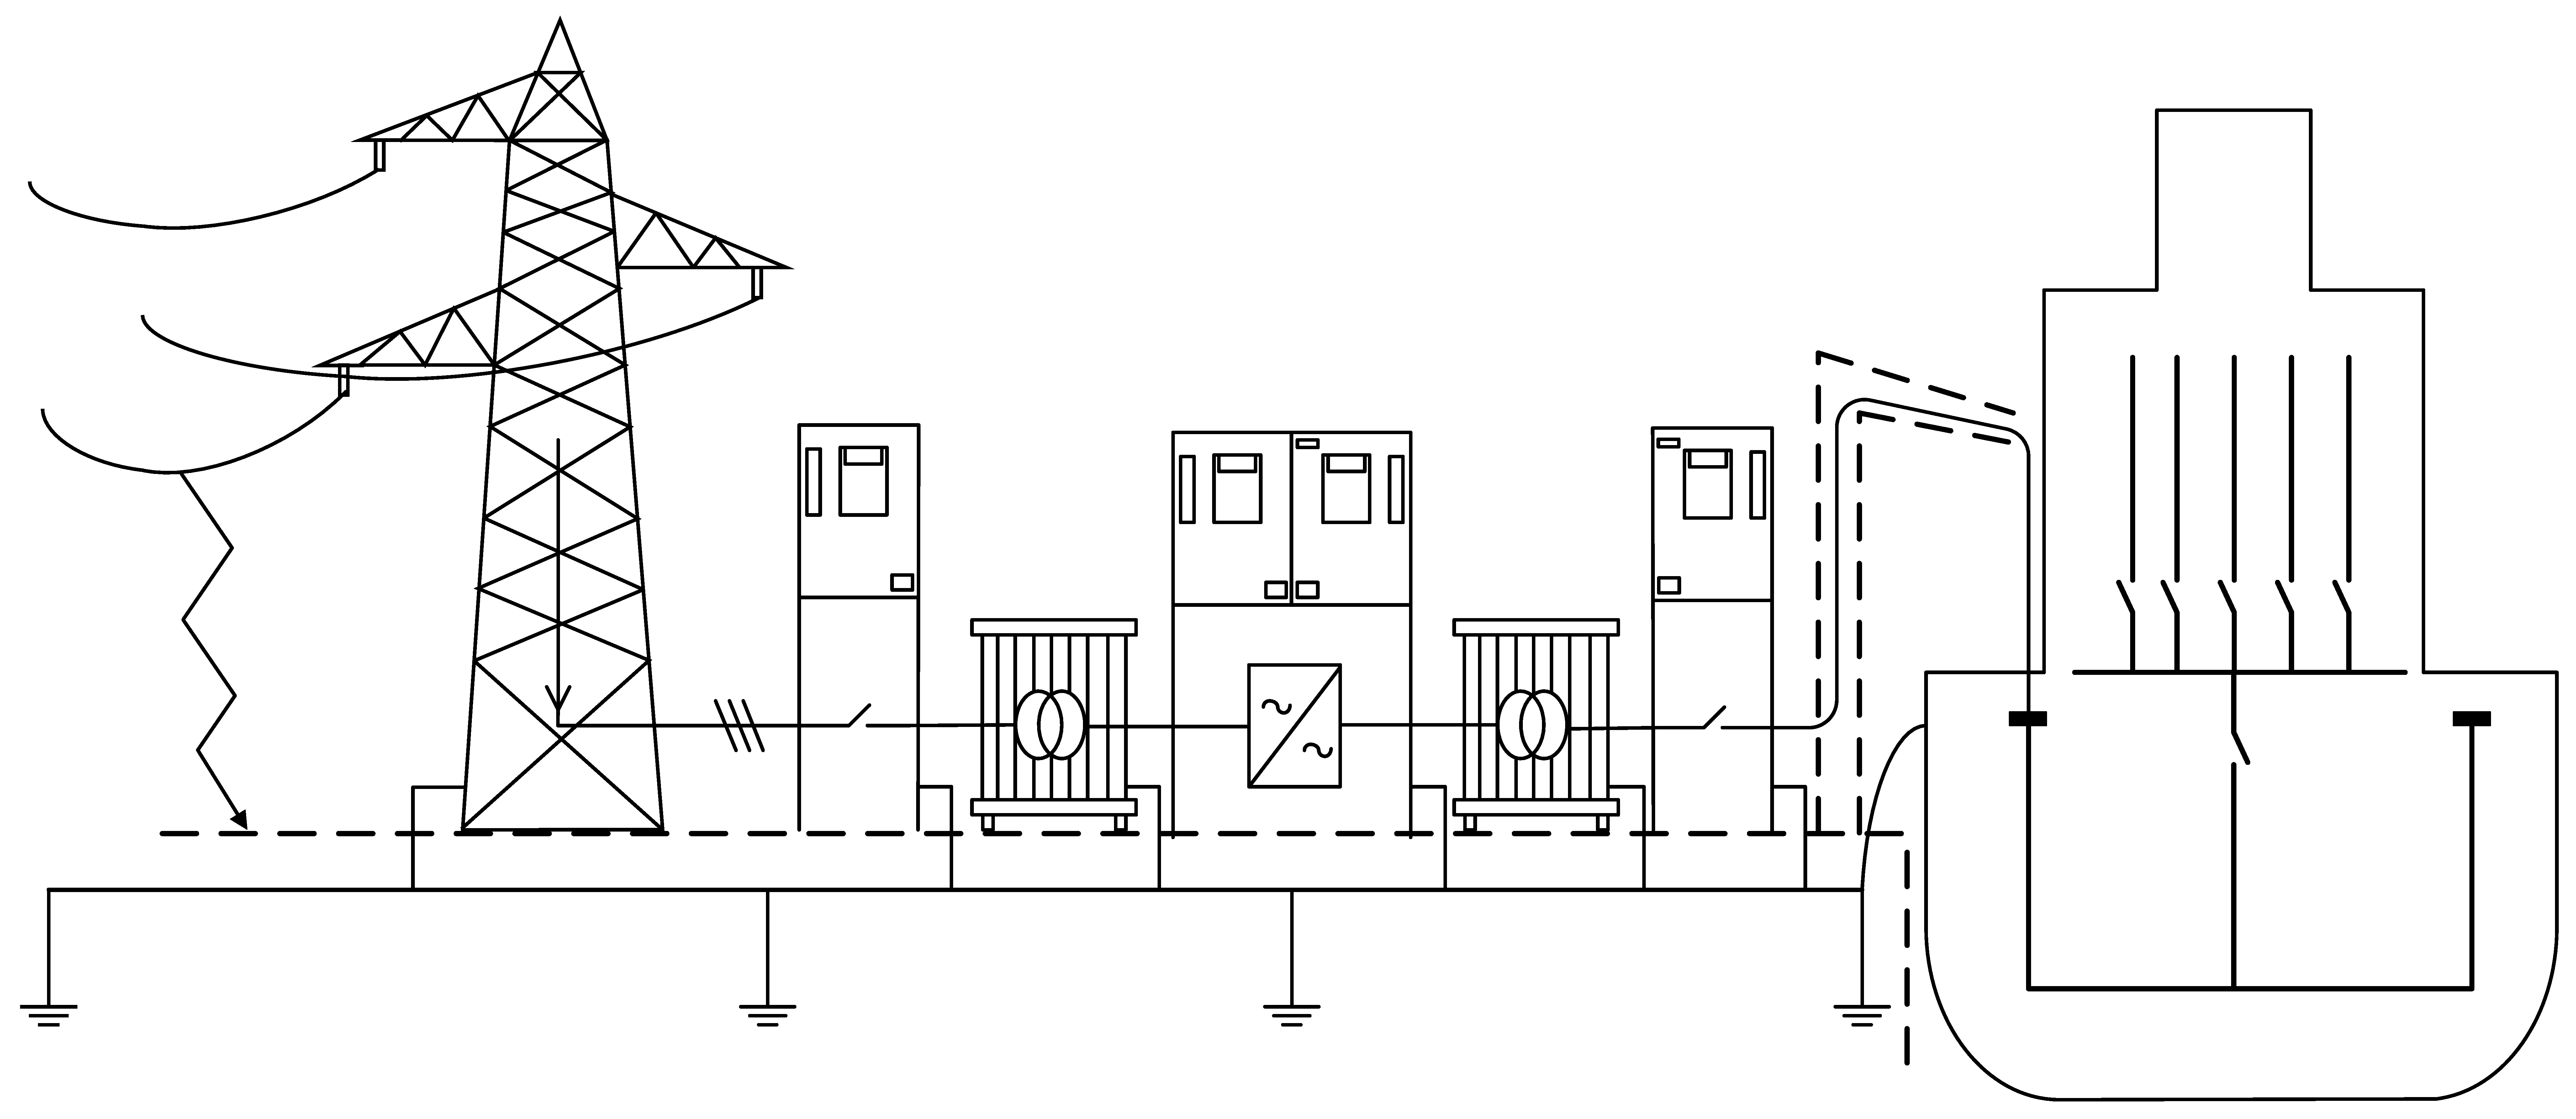
\includegraphics[width=0.95\textwidth]{chapter2/船岸连接系统示意图.pdf}
	\caption{船岸连接系统示意图}
	\label{fig:船岸连接系统示意图}
\end{figure}

岸侧供电系统负责将高压变电站的电力传输到泊位附近的连接点,即终端配电箱,以不间断的方式在船舶电力接收系统之间切换等。首先通过变压器将电网高压转换为低压。
随后,变流系统将对网侧电压变压变频,并通过变压器升至船舶电力系统所需的电压。船岸连接系统应用的电压等级不同,
所需电压由船舶类型决定:一般远洋货轮,大型集装箱船采用高压岸电,小型散货船主要采用低压。

其中,岸电系统的核心部分是岸侧变流系统。国外一些国家的电网(美国、加拿大等),一些客船的电力系统的电网频率通常为60Hz。
在电网频率为60Hz的国家中,船岸连接系统实现变得相对容易,然而在电网频率为50Hz的中国,欧洲诸国与一些其它国家,
为系统岸侧部分提供额外的变频装置是岸电系统所必需的。实现交流电50Hz到60Hz的转变通常有两种解决方案:静态变换器或旋转变换器(图\ref{fig:传统旋转变频与静态电源变频对比})。
考虑到码头的现代全电动邮轮通常需要8–12\si{MW}\cite{SP15},在大容量的船岸连接系统中,岸电变流系统需要满足这种功率需求。
同时,可以承受足够的短路电流使安装在船舶上的继电保护系统能够正常发挥作用。

\begin{figure}[!htp]
	\centering
	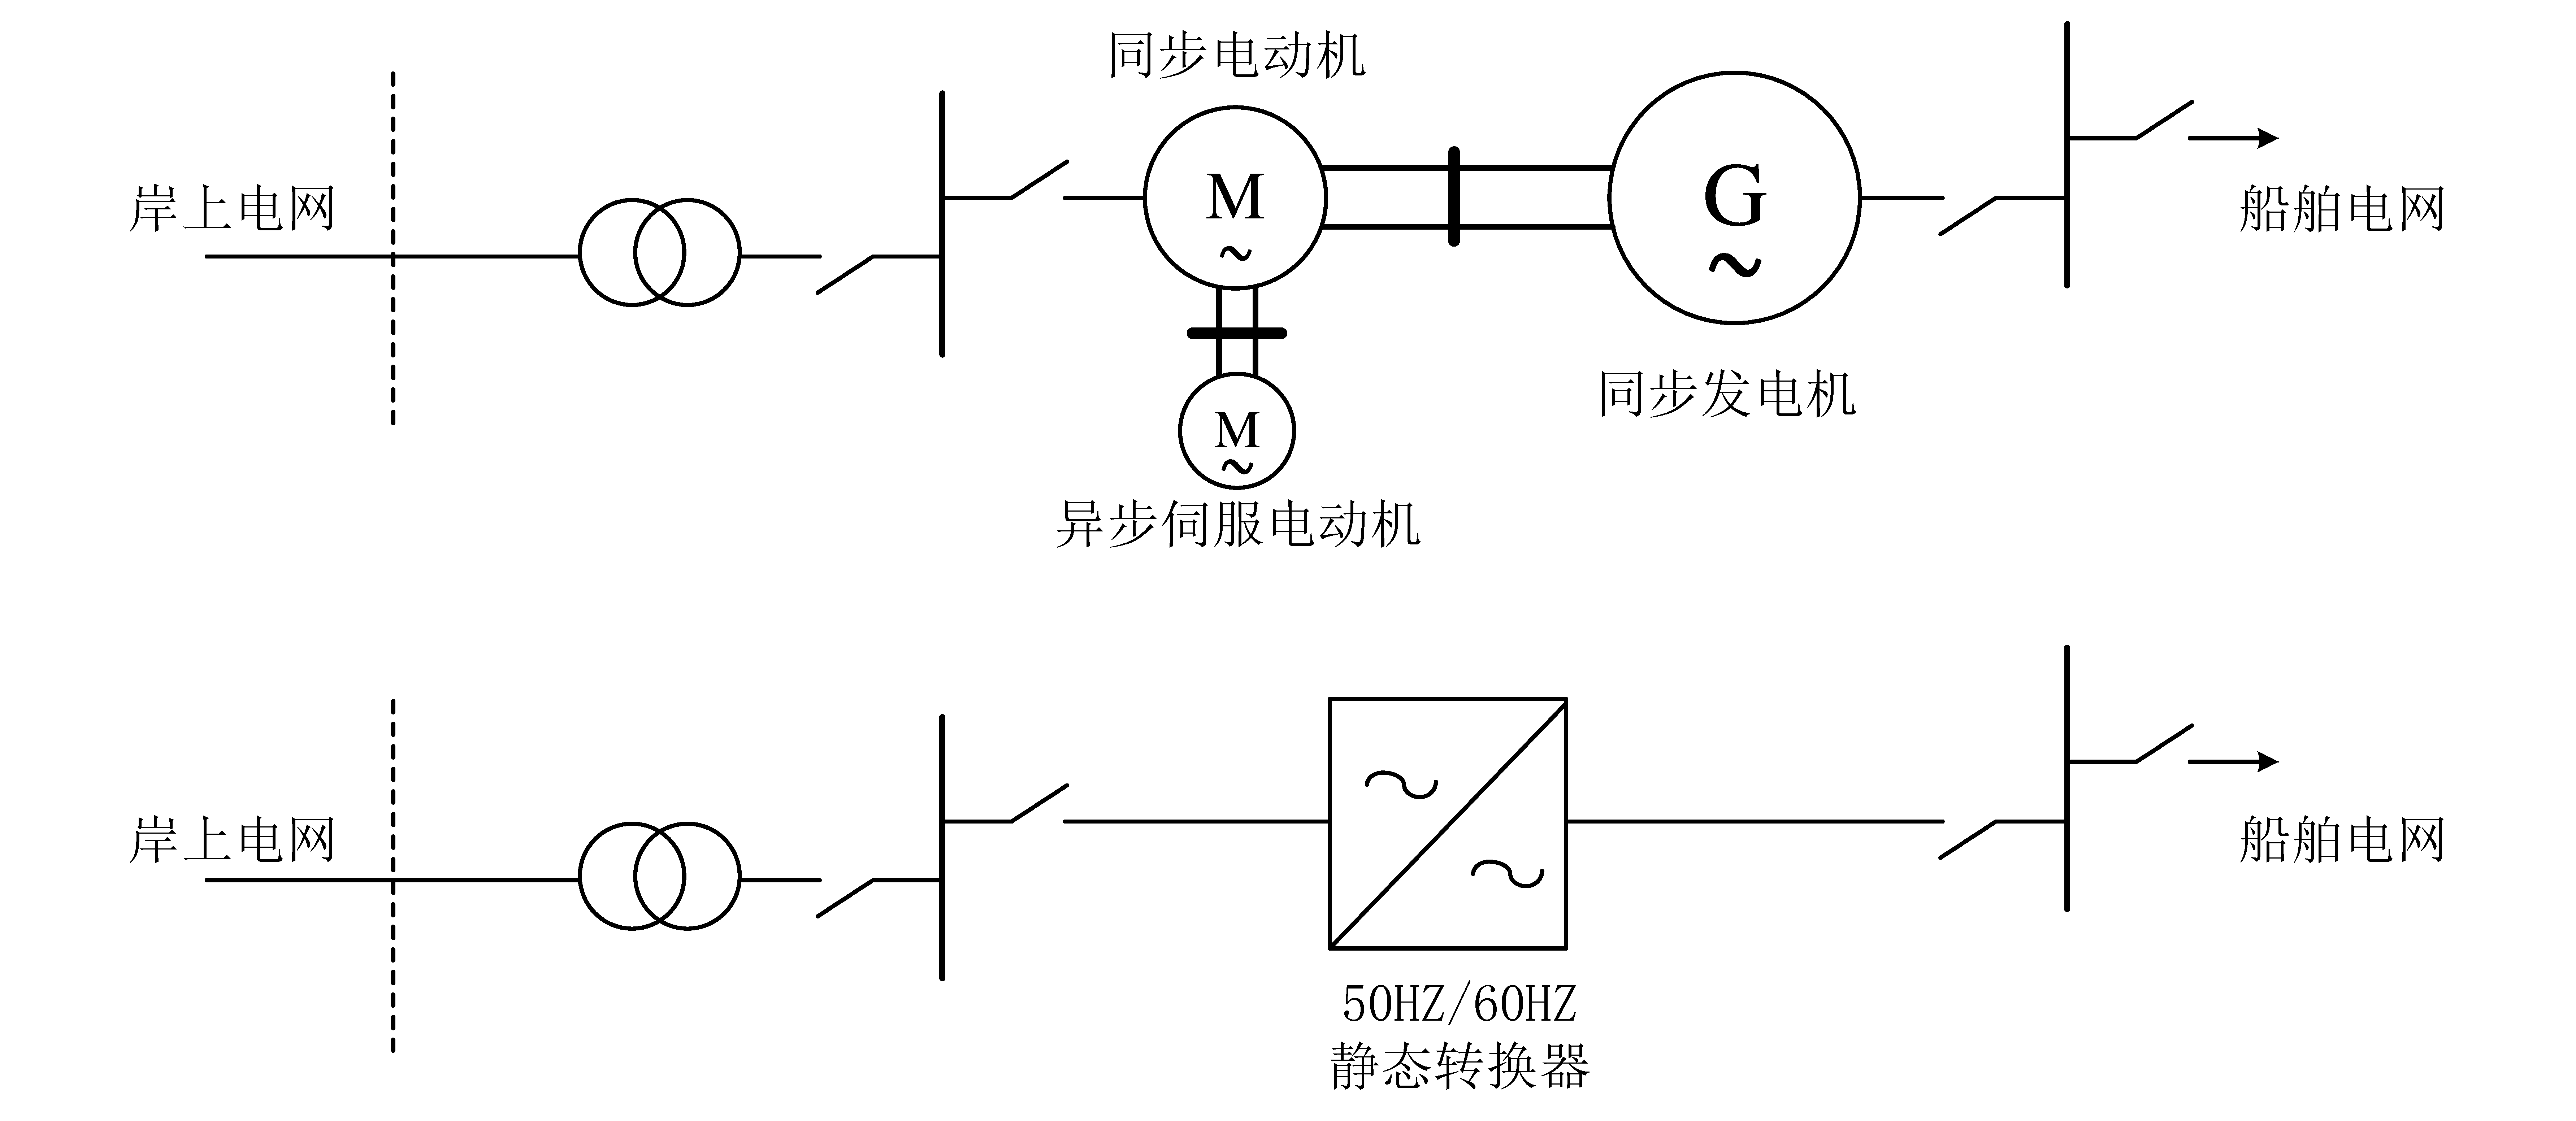
\includegraphics[width=0.85\textwidth]{chapter2/旋转形态转换器对比.pdf}
	\caption{旋转变频与静态电源变频}
	\label{fig:传统旋转变频与静态电源变频对比}
\end{figure}

电缆管理系统包括连接岸侧连接点、船载受电设备的电缆和设备。电缆连接设备必须满足电缆的收放功能,与快速连接的能力,
不使用时应存放在船上、岸上或者驳船上。

\begin{figure}[!htp]
	\centering
	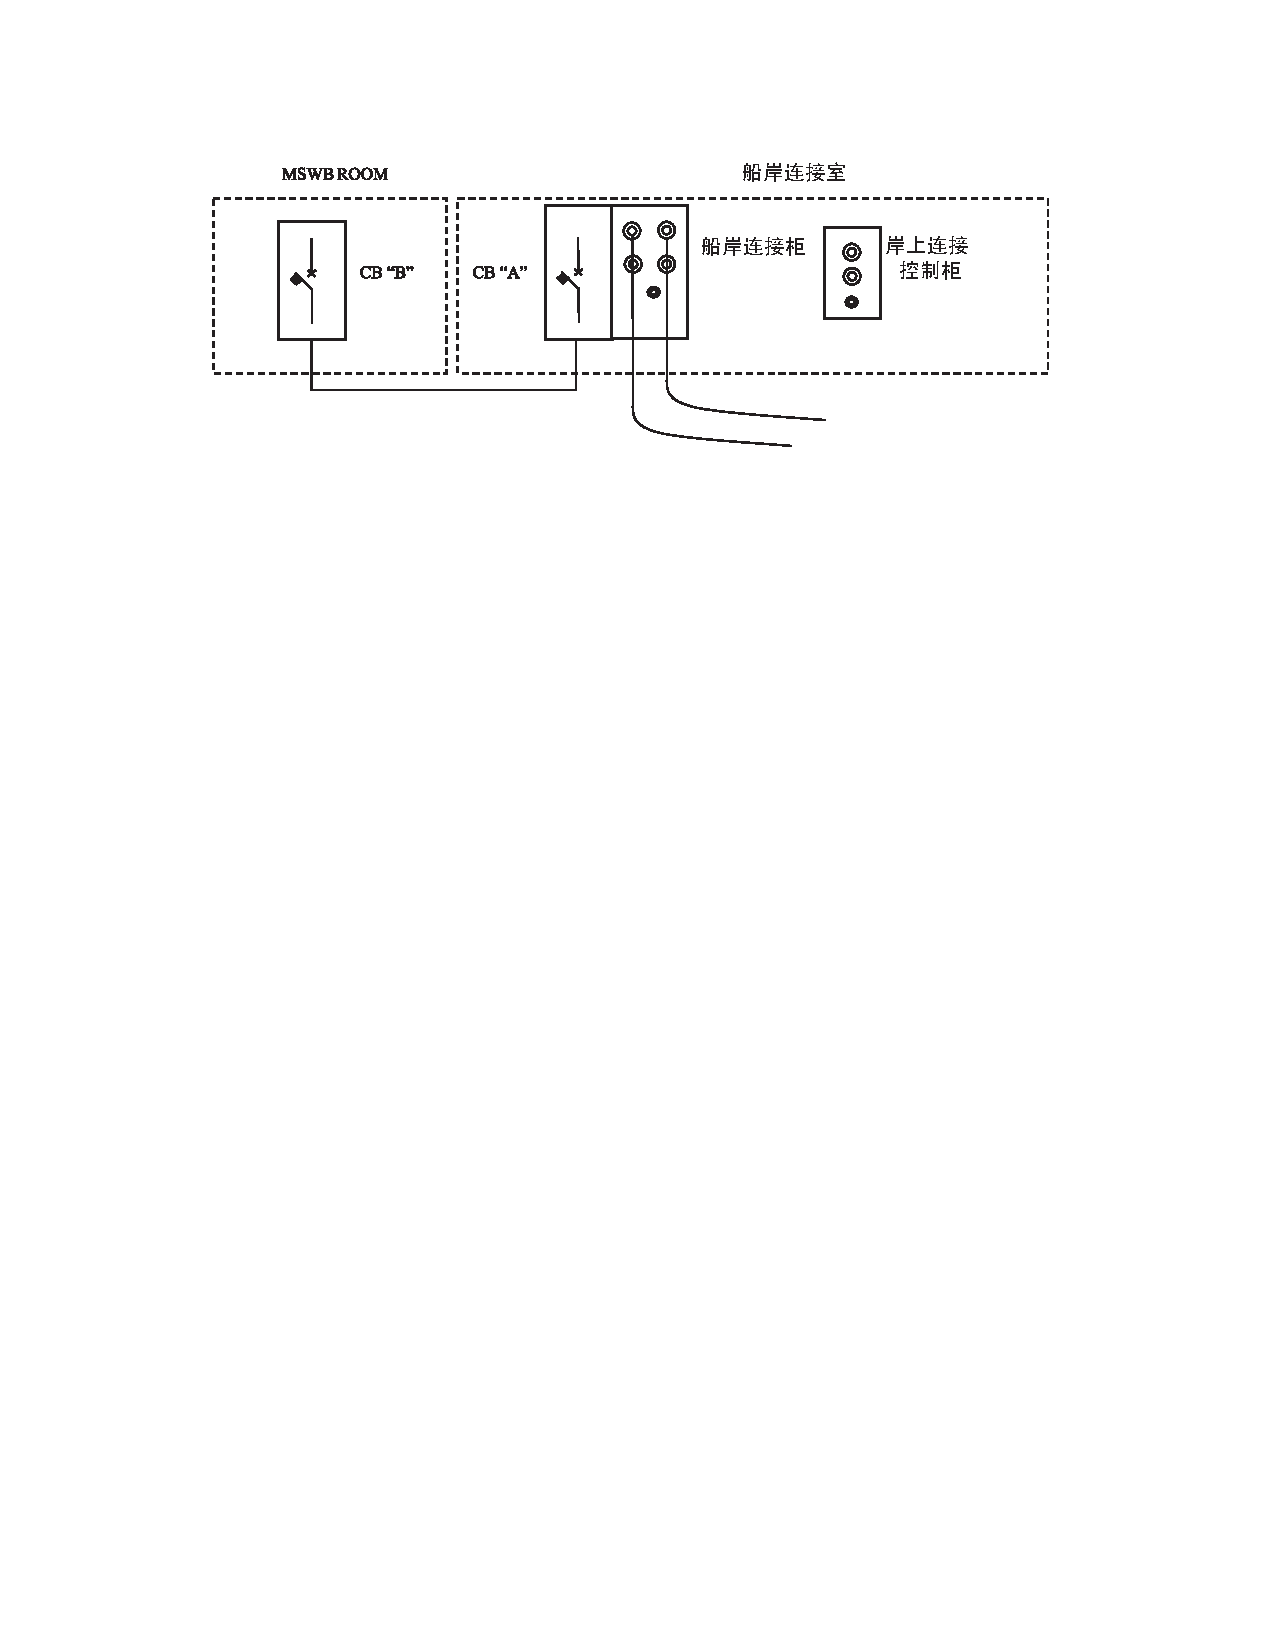
\includegraphics[width=0.85\textwidth]{chapter2/船侧船岸连接部分.pdf}
	\caption{船侧连接系统}
	\label{fig:船侧连接系统}
\end{figure}

如图\ref{fig:船侧连接系统}所示,船侧连接系统是在原有的电力系统上增加接受单元,
包括电缆绞车、船舶变压器、并车装置以及相关控制系统等,有需要时还要安装船舶变频器\cite{SP15}。

此外,船岸连接系统应配备有电气控制系统,监控和报警统和通讯系统。
一种高压岸电电气一次系统,如图\ref{fig:船舶岸电系统一次图}所示。
一次系统由:1.电源进线柜 2.PT柜 3.变频进线柜 4.变频出线柜 5.输出PT柜 6.输出计量柜 7.出线柜组成。

\begin{figure}[!htp]
	\centering
	\includegraphics[width=\textwidth]{chapter2/船舶岸电系统一次图.pdf}
	\caption{船舶岸电系统一次图}
	\label{fig:船舶岸电系统一次图}
\end{figure}

\section{船岸连接系统的分类}

我国的港口分为内河(河、湖)港、江港、海港,所停靠船舶种类多。图\ref{fig:远洋和内河主要船舶类型}中的四种船舶
是远洋或者内河船的一些主要类型。国内船舶的电网电压等级和电压频率一般与国家电网一致,
可直接从电网供电\cite{SP16};国外船舶电压频率一般是60Hz,高压为6.6kV低压为440V,其电制与国家电网不同,不可以
直接从电网供电,必须使用变流装置将变压变频频率,才可以给船舶供电。

\begin{figure}[!htp]
	\centering
	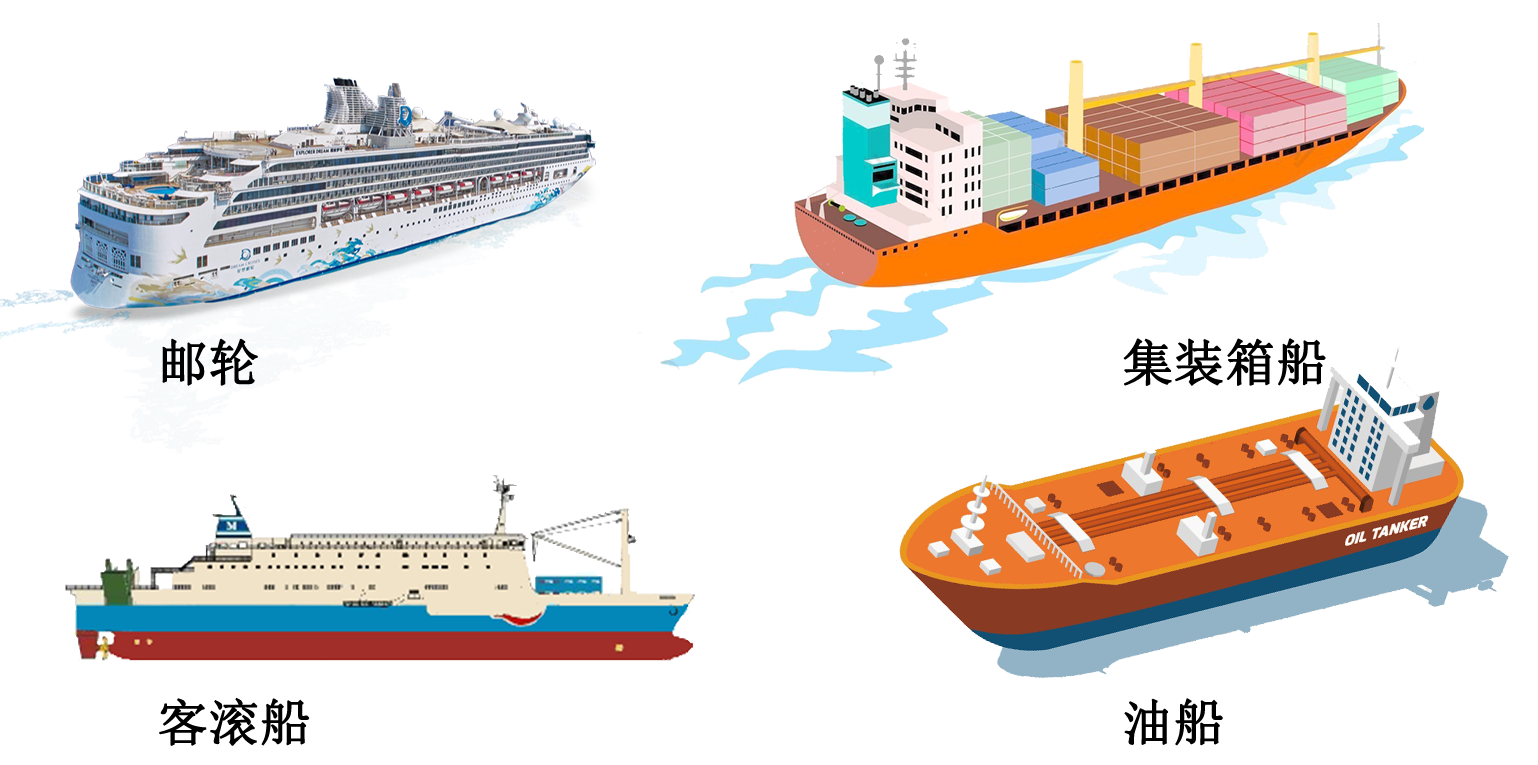
\includegraphics[width=0.75\textwidth]{chapter2/船舶类型.png}
	\caption{远洋和内河主要船舶类型}
	\label{fig:远洋和内河主要船舶类型}
\end{figure}

根据船舶电网的电压等级可以将船舶分为低压船舶和中压船舶。一般将船舶电网电压为440V\~{}690V的船舶划分为低压船舶,
而船舶电网电压为6.6kV\~{}11kV的船舶划分为中压船舶。中压船舶船载电站的电压等级包括11kV、6.6kV(60Hz)和6kV(50Hz),
低压船舶船载电站的电压等级包括400V(50Hz)和440V(60Hz)\cite{SP15}。在岸电系统的电压等级划分上与船舶电网电压等级划分有所区别,
电压在6.6kV\~{}11kV的岸电系统属于高压岸电系统。

文献\cite{SP6}对图\ref{fig:远洋和内河主要船舶类型}中四类船舶的电制进行了详细统计,图\ref{fig:不同电压在四种船舶中的占比}
和\ref{fig:不同频率在四种船舶中的占比}分别表示不同电压和不同频率的船舶在这四类船舶中的所占比例。
可以看到目前大部分船舶仍在使用低压岸电,6.6kV以上的船舶岸电技术主要应用在大型邮轮和远洋集装箱船上。

\begin{figure}[!htp]
	\centering
	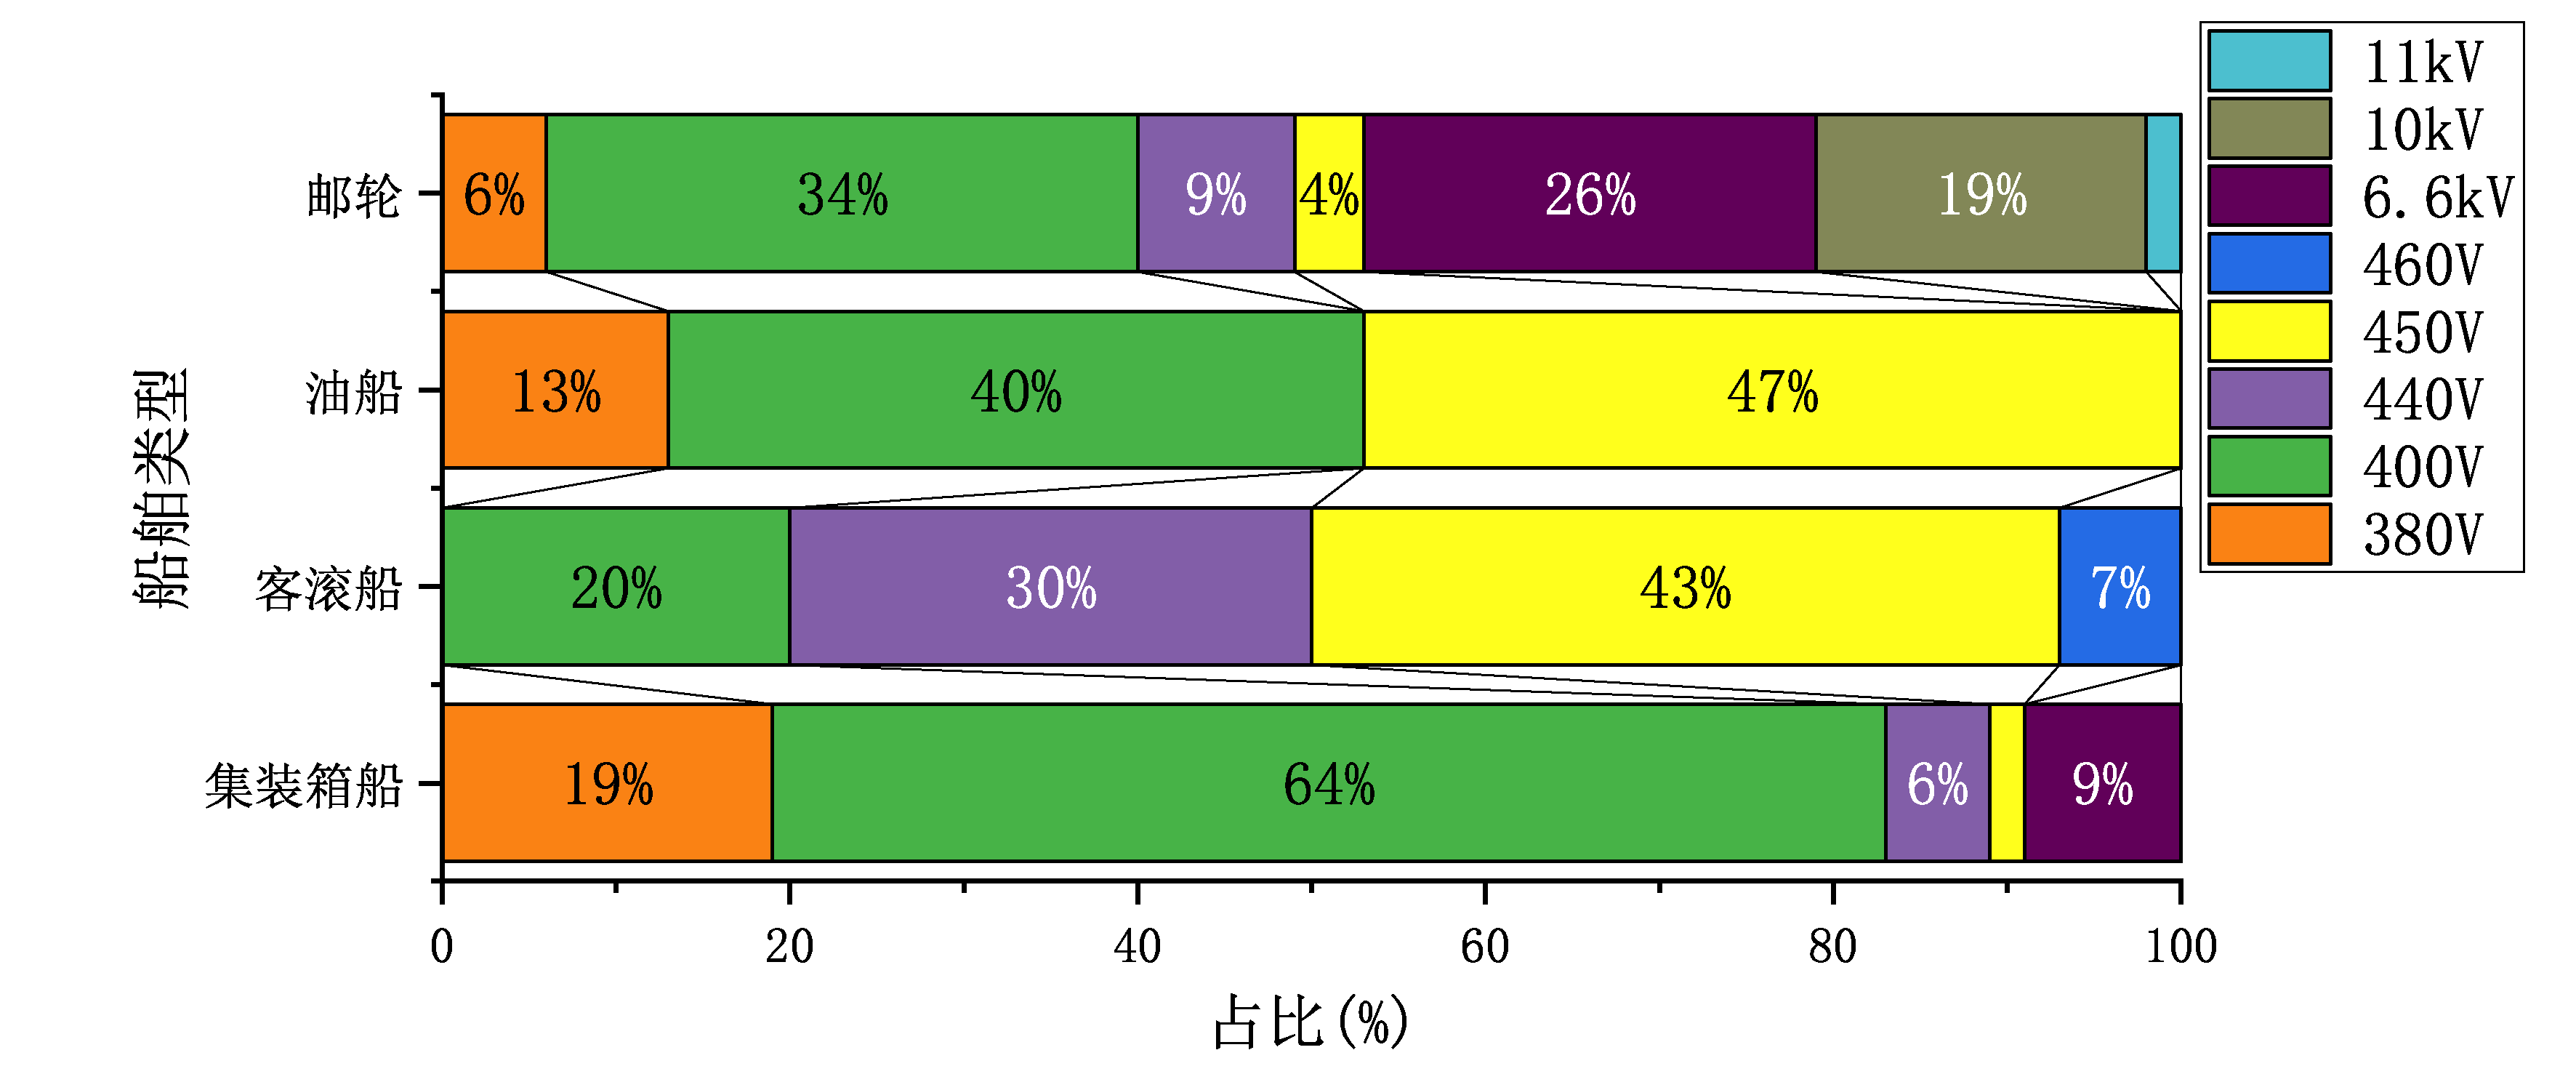
\includegraphics[width=\textwidth]{chapter2/不同电压等级在船舶中占比.pdf}
	\caption{不同电压在四种船舶中的占比}
	\label{fig:不同电压在四种船舶中的占比}
\end{figure}

船舶采用60Hz的交流电是目前的主流方式,不过也不能够因此忽视国内一些采用50Hz频率的船舶。

\begin{figure}[!htp]
	\centering
	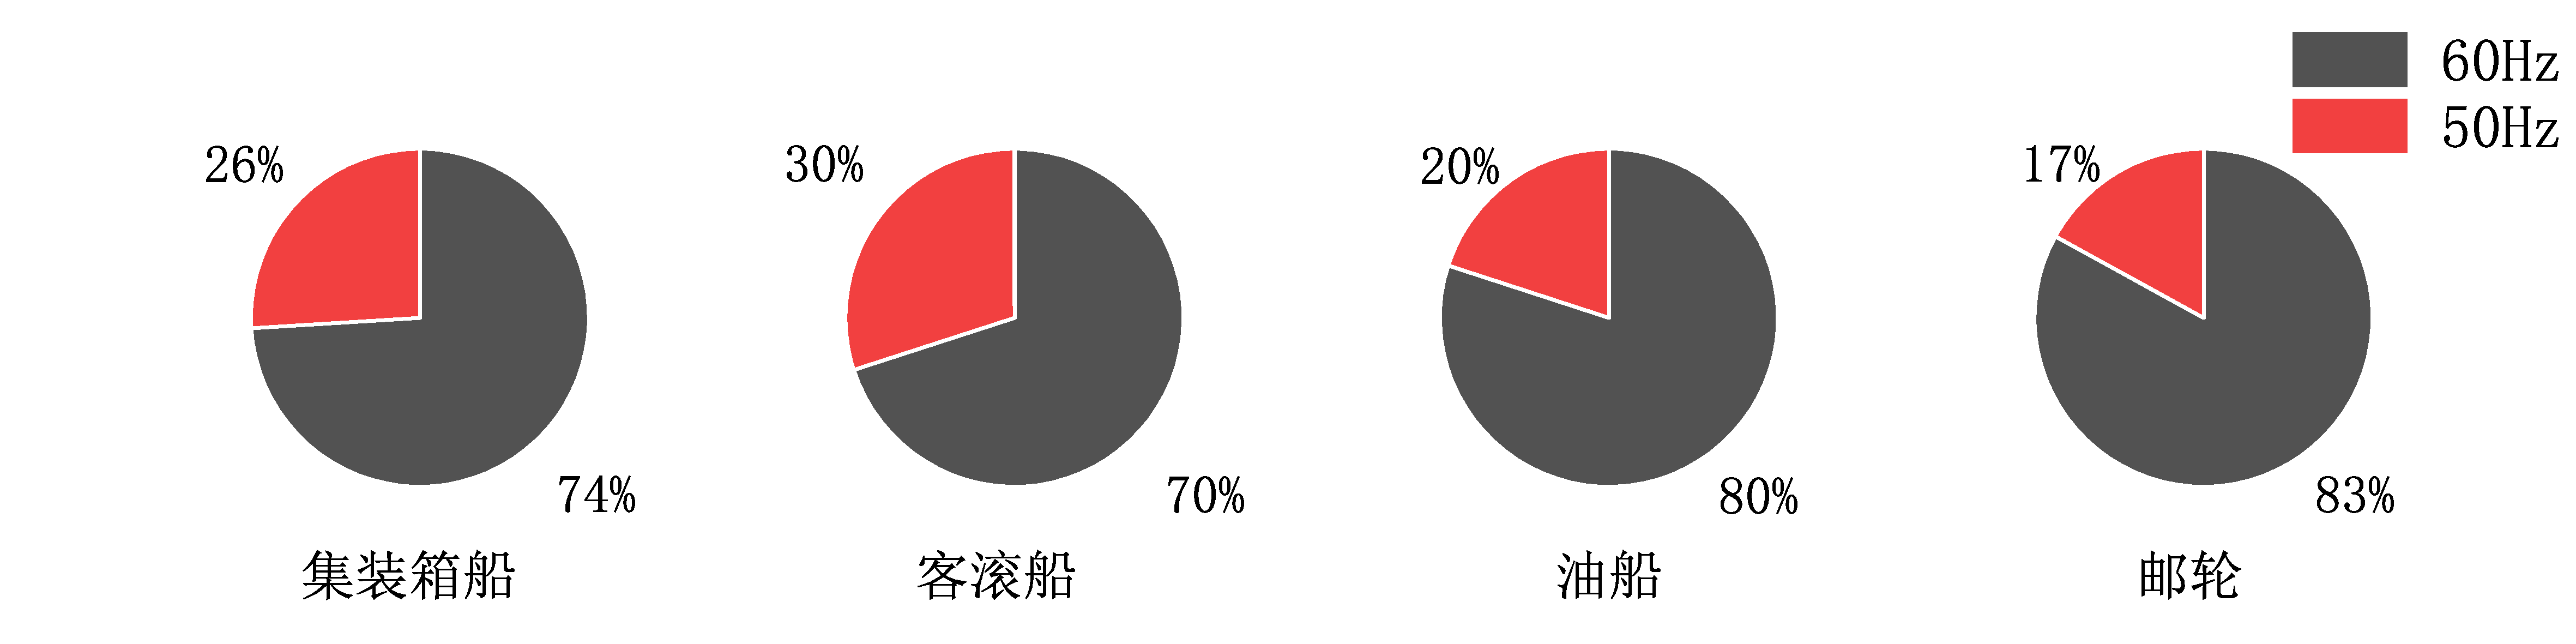
\includegraphics[width=\textwidth]{chapter2/不同频率在船舶中占比.pdf}
	\caption{不同频率在四种船舶中的占比}
	\label{fig:不同频率在四种船舶中的占比}
\end{figure}


为港口建设船岸连接系统应该充分考虑船舶电制、泊位类型和船舶负载容量,根据港口自身情况合理选择适合的岸电系统产品。
表\ref{tab:靠港船舶功率需求}总结了不同类型船舶的功率需求\cite{SP6},由此可见,由于船舶功能初见的多样化
使得船舶负载功率也逐渐增大,有的甚至达到了兆瓦级的功率需求。
根据船舶不同的用电需求,可以将岸电系统应用分为高压岸电供电系统、低压岸电供电系统及小容量岸电供电系统,三类岸电应用形式。

% Table generated by Excel2LaTeX from sheet 'Sheet6'
\begin{table}[htbp]
	\centering
	\caption{靠港船舶功率需求}
	  \begin{tabular}{ccc}
	  \toprule
	  船舶种类  & 功率    & 最高功率 \\
	  \midrule
	  邮轮    & 800kW & 8000kW \\
	  油船    & 1500kW & 2000kW \\
	  客滚船   & 1400kW & 2700kW \\
	  集装箱船  & 5800kW & 11000kW \\
	  \bottomrule
	  \end{tabular}%
	\label{tab:靠港船舶功率需求}%
  \end{table}%
  

\subsection{高压岸电供电系统}

高压岸电供电系统结构如图\ref{fig:高压岸电供电系统}所示,应用在沿海大型港口和码头,具有为负载容量超过800kVA靠港
船舶提供电力的能力\cite{SP16},高压岸电系统典型的容量有:800kVA、1000kVA、2000kVA、3000kVA、5000kVA、
和8000kVA等。
主要由:
1. 岸电电源系统
2. 隔离变压器带接地电阻
3. 保护继电器(岸侧)
4. 高压开关带接地开关
5. 电源控制箱(岸侧)
6. 连接电缆及接口设备
7. 电源控制箱(船侧)
8. 保护继电器(船侧)
9. 船上岸电源接线箱
10. 船上变压器(如有)
11. 船上受电板
组成。

\begin{figure}[!htp]
	\centering
	\includegraphics[width=0.95\textwidth]{chapter2/高压岸电系统.pdf}
	\caption{高压岸电供电系统}
	\label{fig:高压岸电供电系统}
\end{figure}

高压岸电系统(HVSC)采用的是高压上船的模式,将电网10kV或6kV的50Hz电源变压变频后转换为6.6kV或6kV的60Hz或50Hz的高压电。
变频装置一般安装在码头配电室中,通过电缆将电输送至码头泊位的高压岸电接电桩。一般而言,采用高压岸电可以减少
电缆的使用,最少只需一根或两根电缆就可以为船舶提供电力,不过对目前许多船舶,使用高压岸电的成本比较高,需对船舶本身
进行改造,配置相关设备。

\subsection{低压岸电供电系统}

低压岸电供电系统(LVSC)结构如图\ref{fig:低压岸电供电系统}所示,一般应用在,内河港,江港的码头,系统提供的用电容量一般不高于
800kVA。采用低压岸电的方案时,如果船舶用电需求高于400kVA,需要连接的低压电缆数量多,电缆连接难度大,时间长,所以
低压岸电系统典型的容量有:200kVA、400kVA、630kVA、800kVA、1250kVA、1600kVA和2000kVA。
当船舶负载容量大于400kVA时,推荐采用高压岸电系统。目前,岸电标准IEC 60092-510中规定岸电电源提供的电压等级是6.6kV
或11kV,高压岸电系统是船舶岸电发展的主要方向。 
主要由:
1. 岸电电源系统
2. 隔离变压器带接地电阻/ IT 系统
3. 保护继电器(岸侧)
4. 低压主开关
5. 低压出线开关
6. 电源控制箱(岸侧)
7. 连接电缆及接口设备
8. 电源控制箱(船侧)
9. 保护继电器(船侧)
10. 船上岸电源接线箱
11. 船上变压器(如有)
12. 船上低压受电板
组成。

\begin{figure}[!htp]
	\centering
	\includegraphics[width=0.95\textwidth]{chapter2/低压岸电系统.pdf}
	\caption{低压岸电供电系统}
	\label{fig:低压岸电供电系统}
\end{figure}

低压岸电系统采用的是低压上船的模式,将电网10kV或6kV的50Hz电源变压变频后转换为440V(60Hz)或400V(50Hz)的低压
电源。一些不停靠60Hz船舶的内陆港口,可以不用安装变频装置,船上用电设备可以直接使用电网供电。需要停靠60Hz低压
船舶时,一般将变压变频装置放在码头配电室中,通过电缆将电力输送至码头低压的接电桩。需要接入低压岸电系统的船舶
一般不需要对其进行改造,只需配置相应的电缆连接装置和并车装置即可。

\subsection{小容量岸电供电系统}

小容量岸电供电系统结构如图\ref{fig:低压岸电供电系统}所示,一般应用在小型港口和码头,所提供的用电容量一般小于
20kVA。这类码头一般停靠的是些散货船,一千吨以下的小型船,小容量的岸电供电系统可以为这些停靠在内河、湖泊的船只提供
380V(50Hz)的电源,满足船上生活照明所需电力。

\begin{figure}[!htp]
	\centering
	\includegraphics[width=0.95\textwidth]{chapter2/小容量岸电系统.pdf}
	\caption{小容量岸电供电系统}
	\label{fig:小容量岸电供电系统}
\end{figure}

小容量岸电供电系统是在码头将电网10kV(50Hz)的三相高压交流电经过变压器降压为380V三相低压交流电,停靠在码头的
船只使用电缆连接建在泊位上的小容量的岸电接电桩,一般不需要对船本身进行改造。

\section{船岸连接系统供电模式及对比}

船舶岸电系统所提供的电源有高压和低压的区别,通常低压岸电系统只能够给低压船舶(440V60Hz或400V50Hz)供电,
而高压岸电系统不仅可以为中压船舶(一般为6.6kV60Hz或11kV60Hz)供电,也可以通过二次变换为低压船舶供电。
船岸连接系统供电模式可以分为以下三种类型:

\begin{figure}[!htp]
	\centering
	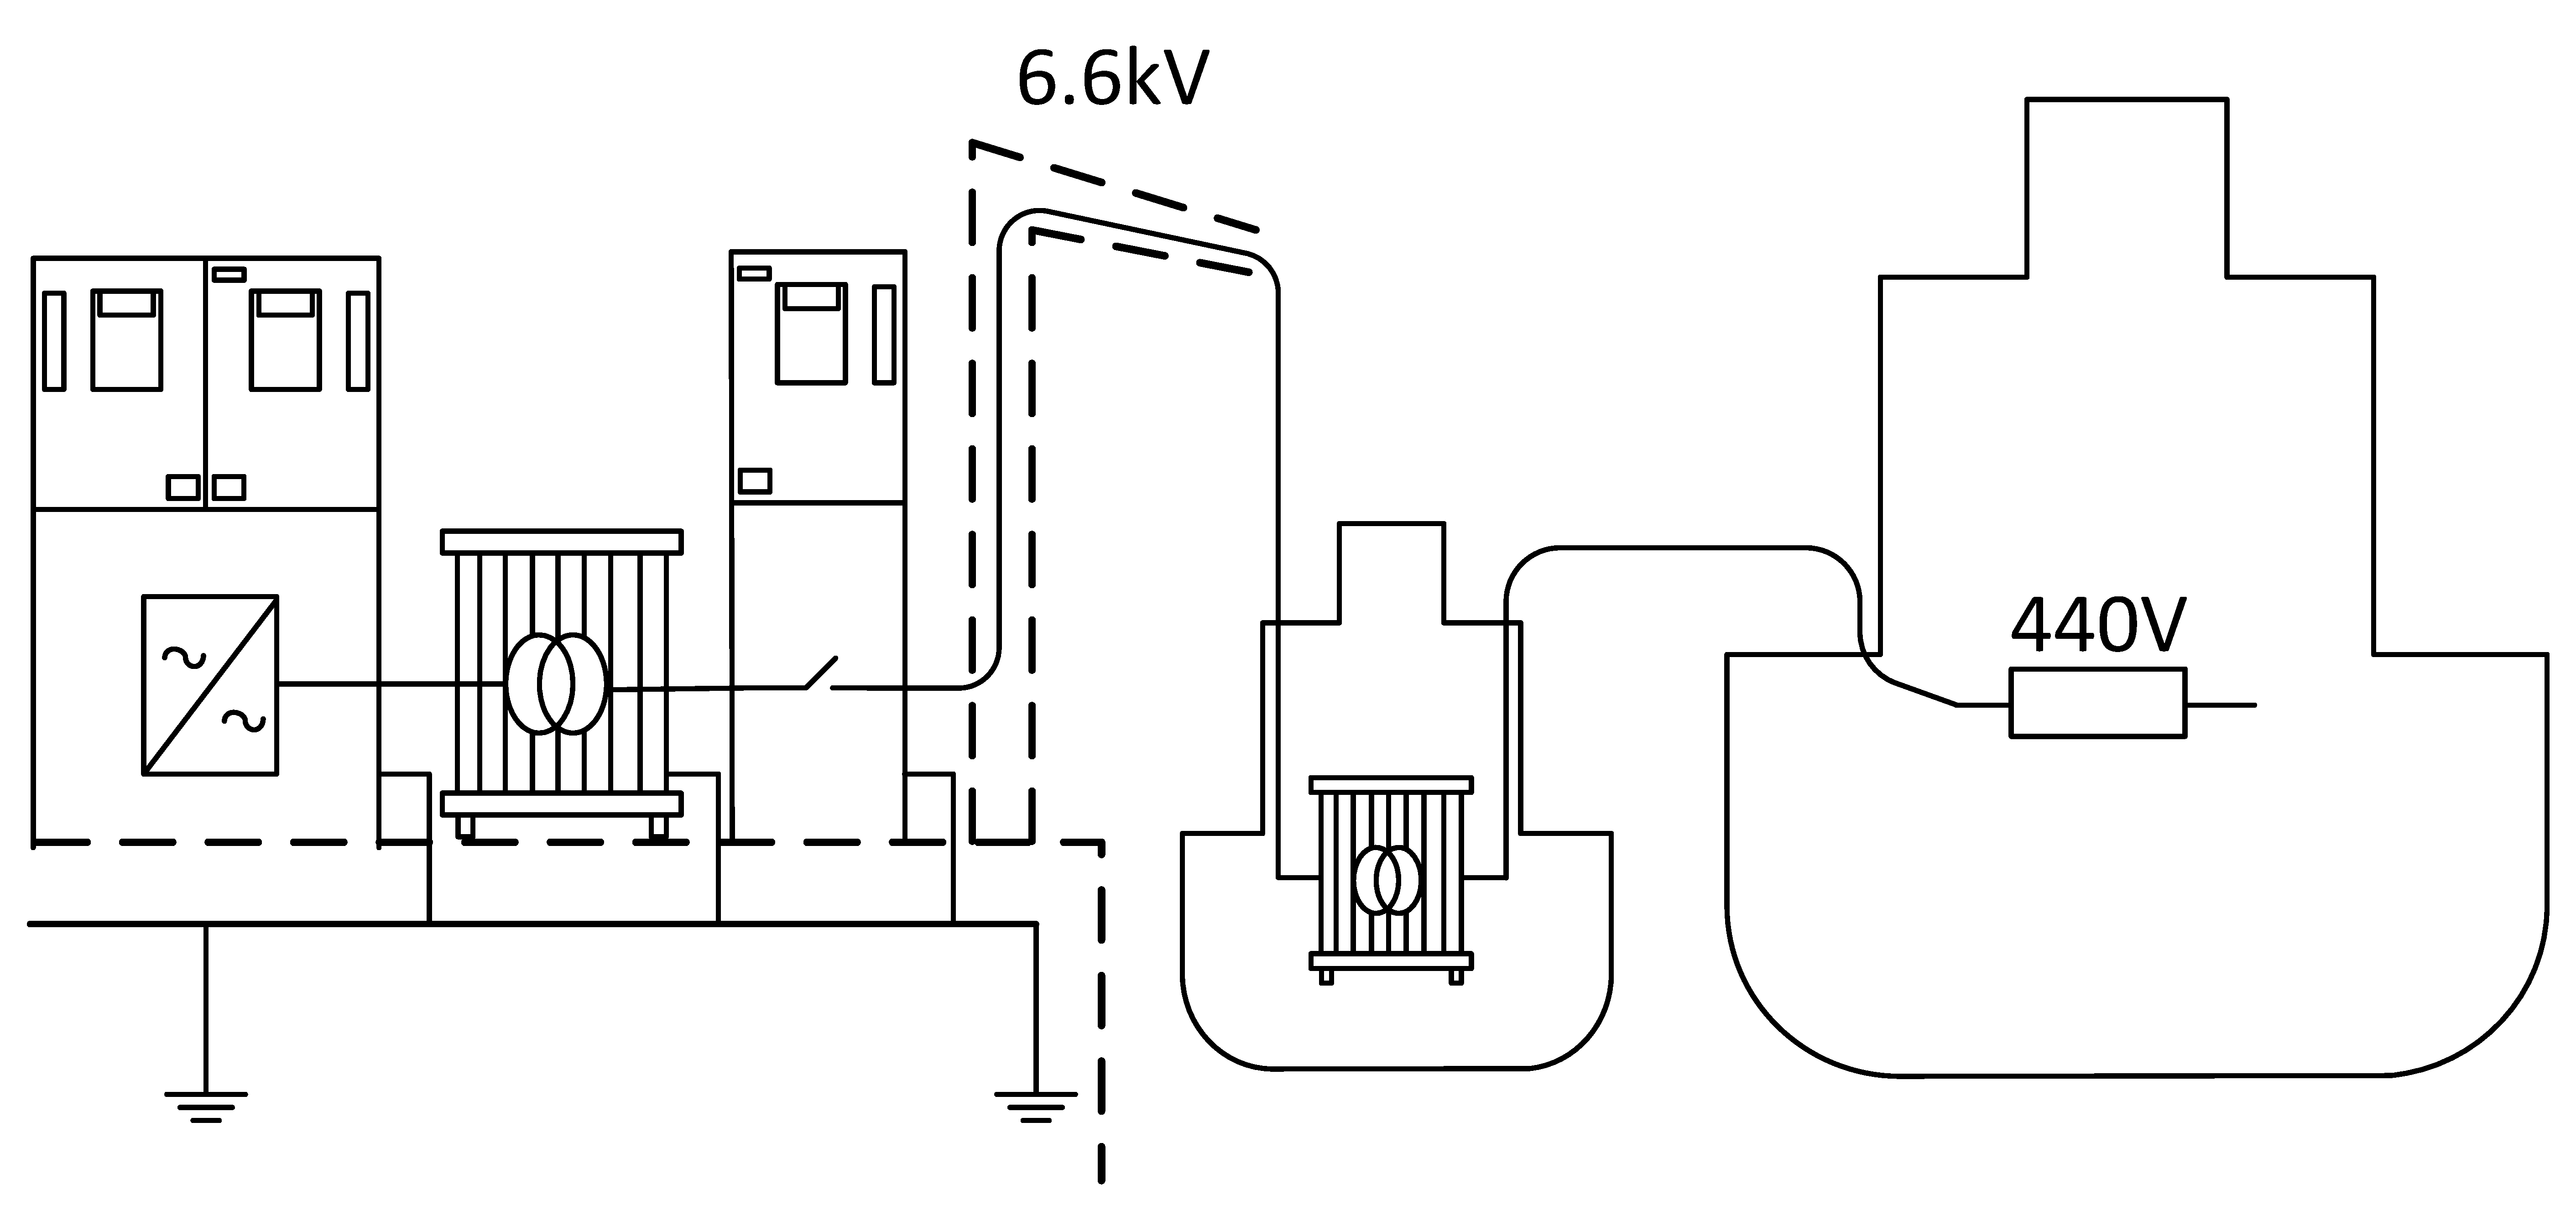
\includegraphics[width=0.7\textwidth]{chapter2/低低.pdf}
	\caption{低压岸电到低压船舶}
	\label{fig:低低}
\end{figure}

(1)低压岸电到低压船舶供电模式如图\ref{fig:低低}所示。
美国洛杉矶港曾采用此种方案,具体过程为:电网高压电经过总变电站输送至变流装置,经变压变流后将至6.6kV60Hz,然后经地下电缆将电力送至码头接线箱。
船舶所需要的电压为440V60Hz,为了节省码头空间,将变压装置放置在泊位与船舶之间的驳船上,驳船连接高压岸电后
经变压器降至440V,船舶则通过电缆连接驳船,从而实现低压岸电到低压船舶的方案。
此种模式需要增加中间的驳船环节,优点是使用时比较灵活,不需要占据码头紧张的空间,缺点也十分明显,
需要多根电缆,连接复杂费时。

(2)高压岸电到高压船舶供电模式如图\ref{fig:高高}所示。
美国长滩港曾使用该方案,具体过程为:电网高压电经过总变电站输送至变流装置,经变压变流后将至6.6kV60Hz,然后经地下电缆将电力送至码头接线箱。
船舶所需要的电压为440V60Hz,然后直接通过电缆连接到船舶,中间不需要降压环节。
此种模式优势明显,只需要一根电缆,因此连接操作简单,连接时间段。缺点是如果用电船舶需要安装岸边变压器
或者船舶变压器。

\begin{figure}[!htp]
	\centering
	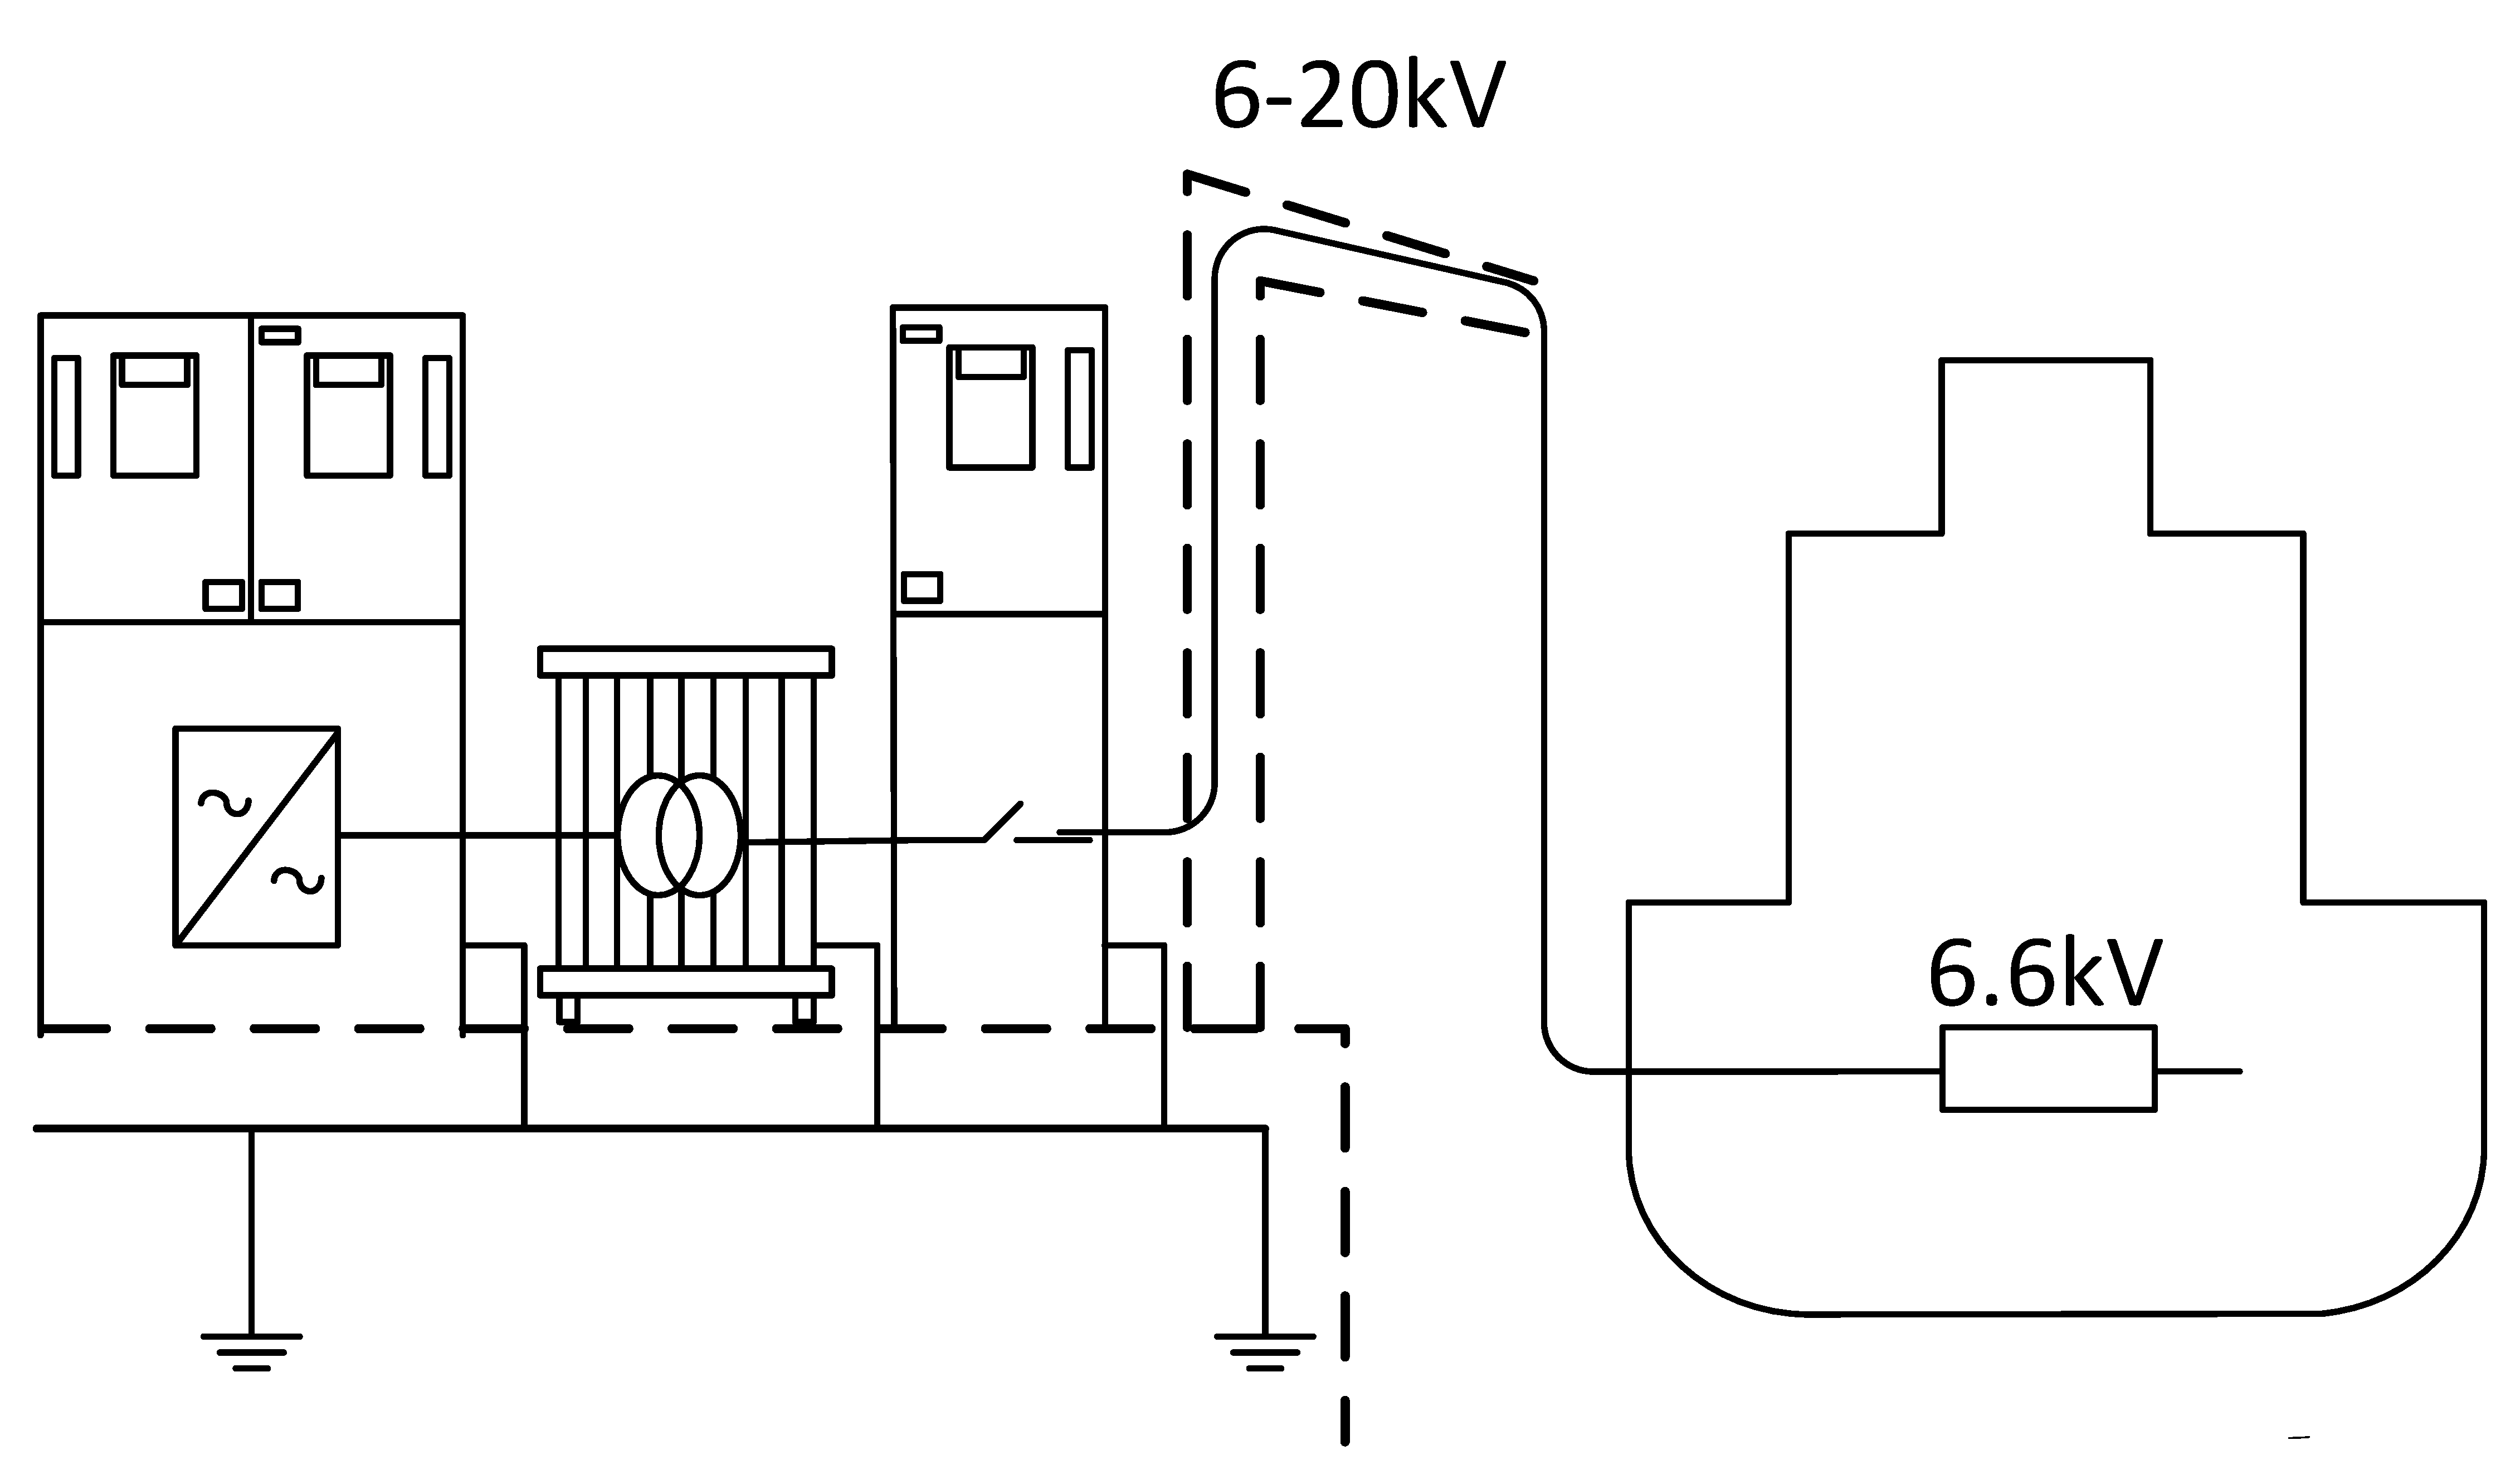
\includegraphics[width=0.6\textwidth]{chapter2/高高.pdf}
	\caption{高压岸电到高压船舶}
	\label{fig:高高}
\end{figure}

(3)高压岸电到低压船舶供电模式如图\ref{fig:高低}所示。
瑞典的哥德堡港作为世界第一个应用高压岸电的港口就采用了此种方案。具体过程为:
电网高压电经过总变电站输送至变流装置,经变压变流后将至6.6kV60Hz,然后经地下电缆将电力送至码头接线箱。
然后只需要一根电缆就可以实现高压上船,因此与前种方案具有同样的优点,缺点是需要对船舶进行改造,成本高。

\begin{figure}[!htp]
	\centering
	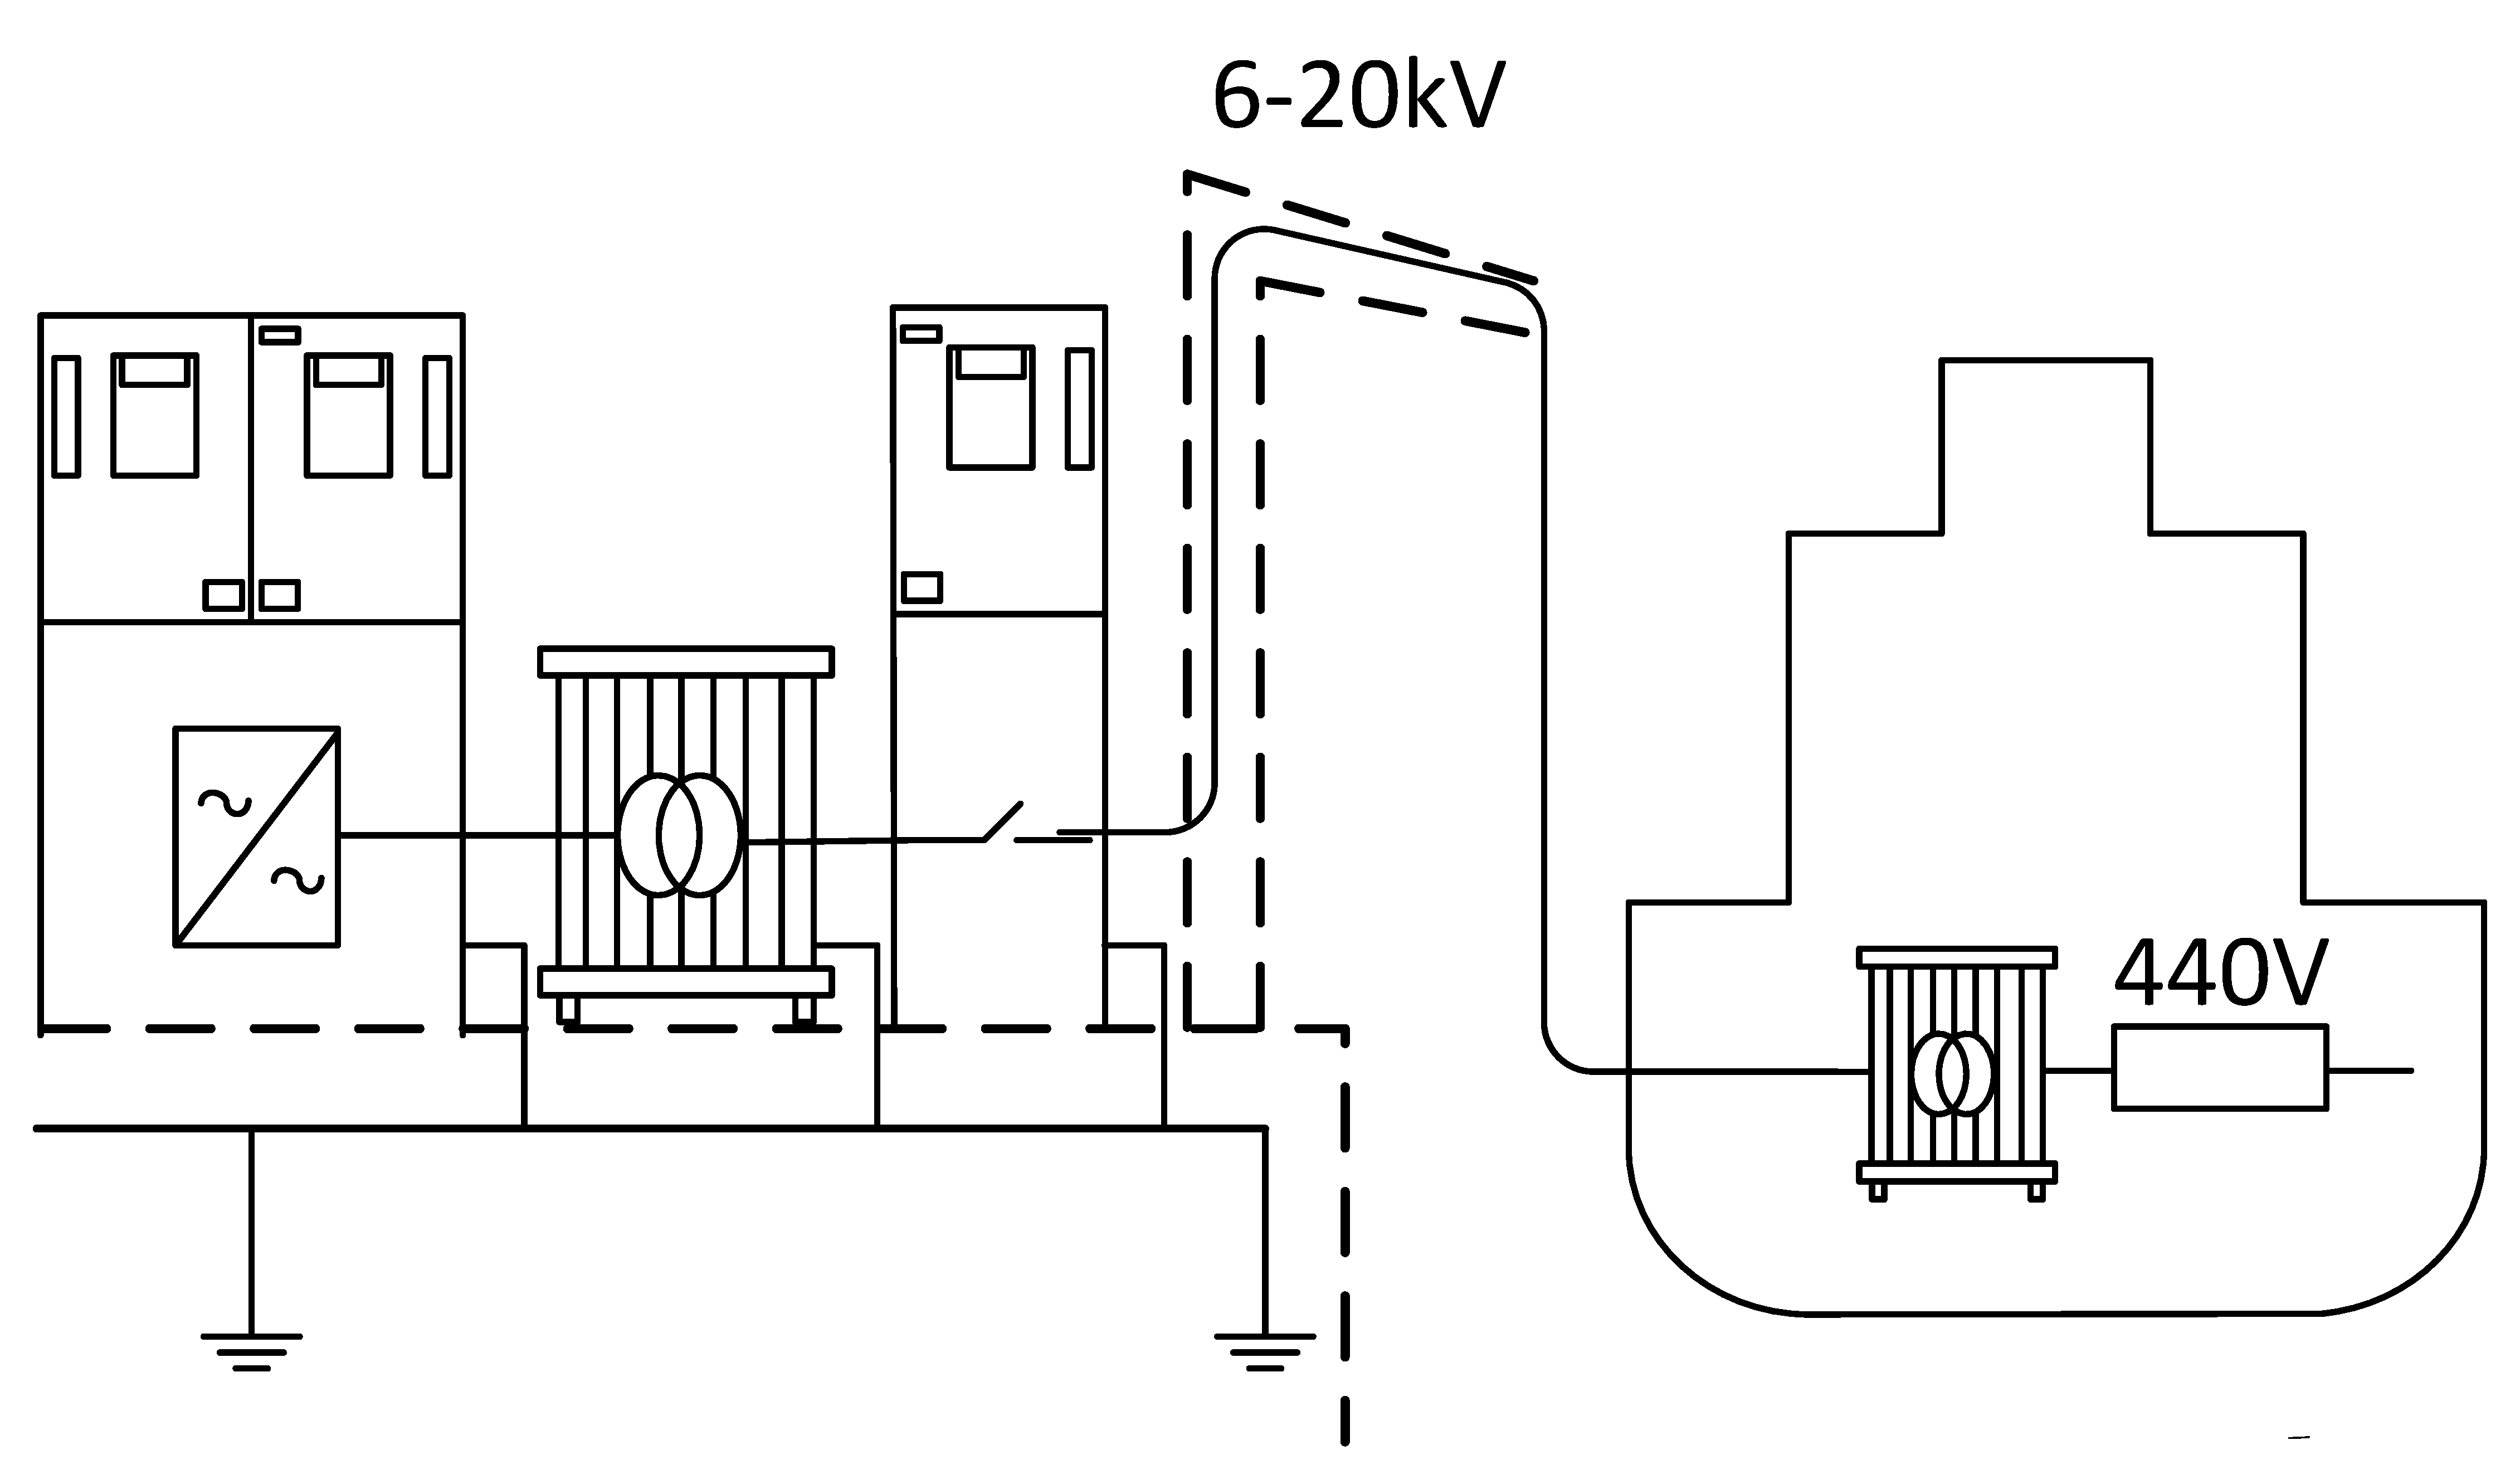
\includegraphics[width=0.6\textwidth]{chapter2/高低.pdf}
	\caption{高压岸电到低压船舶}
	\label{fig:高低}
\end{figure}

以上三种供电方案各有优缺点,通过表\ref{tab:船用岸电供电方式比较}
可以看出,高压供电所需的电缆数量少,连接相对简单,不足的是需要对船侧设备或岸侧设备进行改造,建设成本高。
低压供电所需的电缆数量多,连接相对复杂、耗时,不过无需对船侧和岸侧设备进行改造,建设成本低。

\begin{table}[!htp]
	\centering
	\caption[船用岸电供电方式比较]{船用岸电供电方式比较}
	\label{tab:船用岸电供电方式比较}
	\resizebox{\textwidth}{!}{%
	\begin{tabular}{c}
		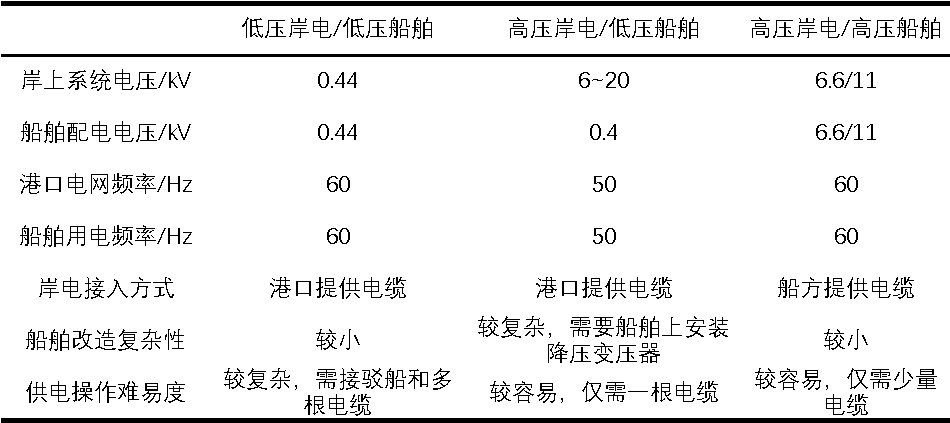
\includegraphics{chapter2/船用岸电供电方式比较.pdf} 
	\end{tabular}
	}
\end{table}

\section{船岸连接系统分布形式}

\subsection{分布式配置形式}

配置形式如图\ref{fig:分布式岸电结构}所示,分布式最大的特点就是每个泊位上都有一个独立的变压器,配备
单独的变频装置,港口总变电站设置有大容量变压器。这种形式的优势在于,系统稳定可靠,多组变频器能够避免
单个变频装置出错时影响整体系统的运行,系统容错率高。这种方式的缺点也十分的明显,港口空间有限,安装
大量的变压变频装置挤占了宝贵的岸上空间,另外该方式的实现也需要大量的资金投入,对港口进行改造。

\begin{figure}[!htp]
	\centering
	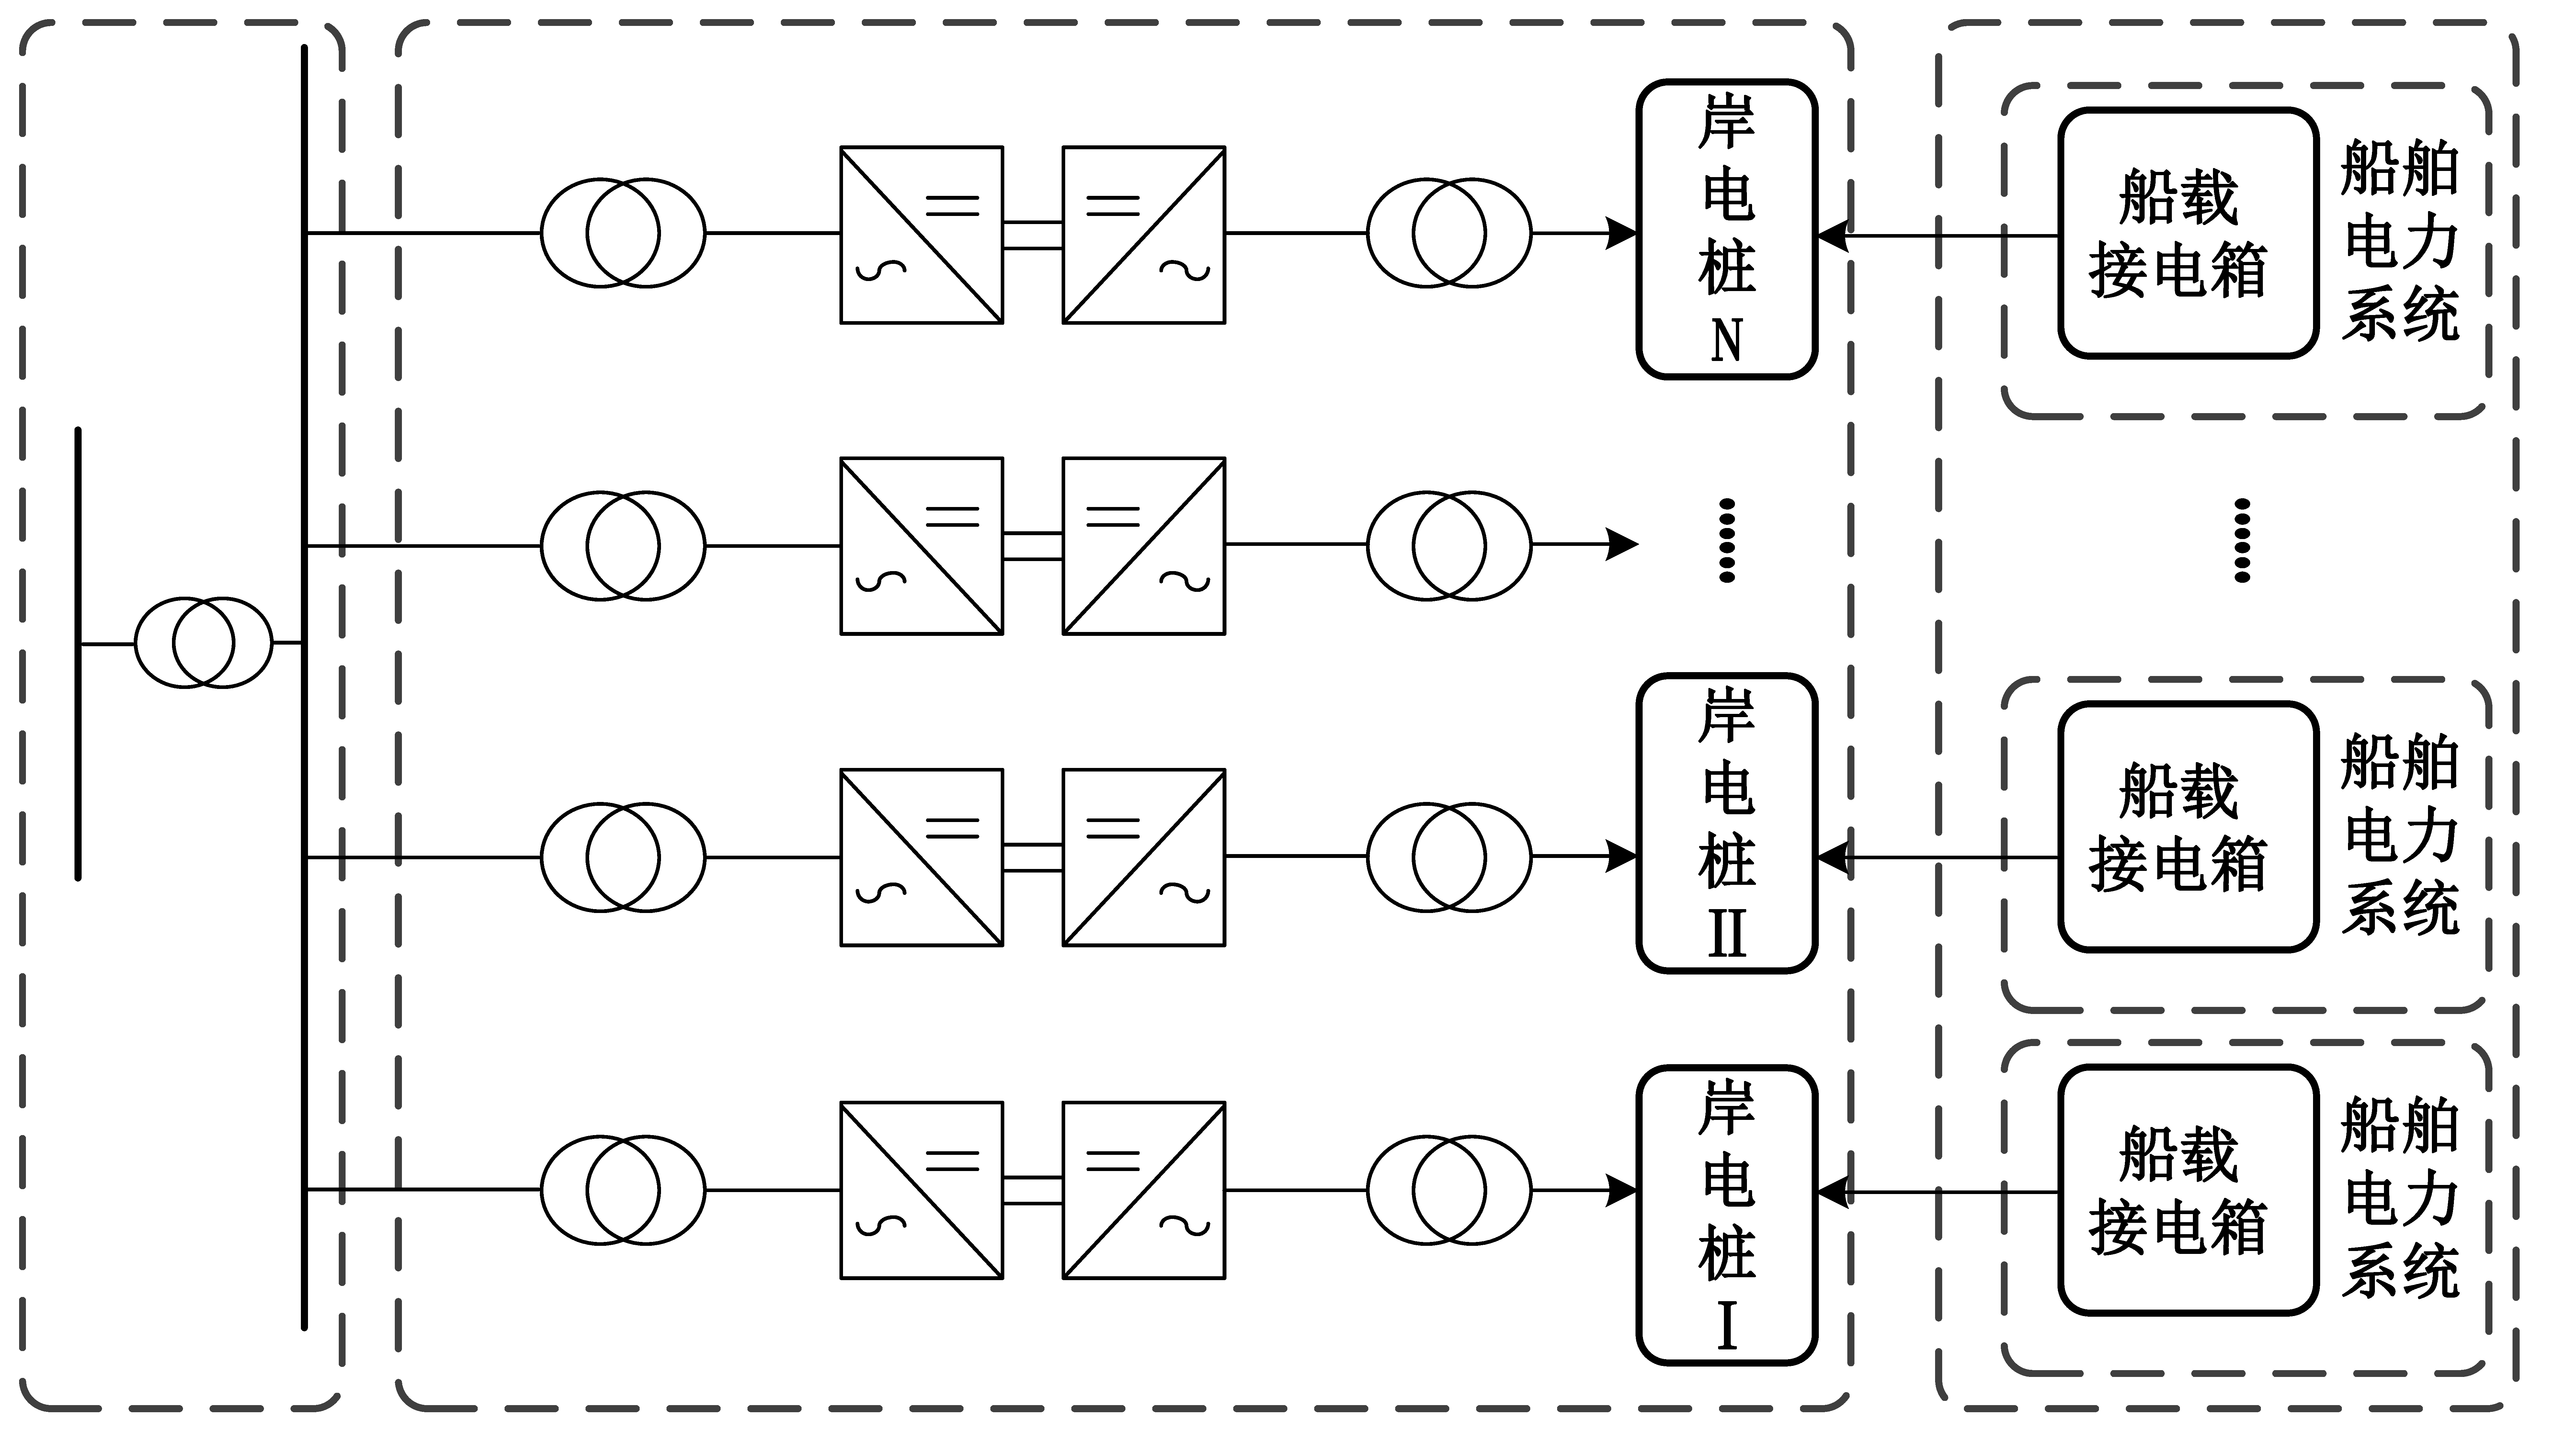
\includegraphics[width=0.85\textwidth]{chapter2/分布式岸电电源.pdf}
	\caption{分布式岸电结构}
	\label{fig:分布式岸电结构}
\end{figure}

\subsection{集中式配置形式}

配置形式如图\ref{fig:集中式岸电结构}所示,与分布式方案不同,岸电系统只需要在主变电站中安装一套变压变频装置。
分两路供电,一路为50Hz不经过变频装置即可向50Hz船舶供电,另一路经过变频装置可以为60Hz船舶供电。
此种方式缺点明显,系统容错性差,当主变频器发生故障时,所有泊位的60Hz岸电接线箱均无法正常工作。
优点是性价比高、岸电建设投入少,不会大量占用宝贵的港口空间。正因集中配置形式的建设优点,此种方式
仍是岸电电源配置的主流方案。

\begin{figure}[!htp]
	\centering
	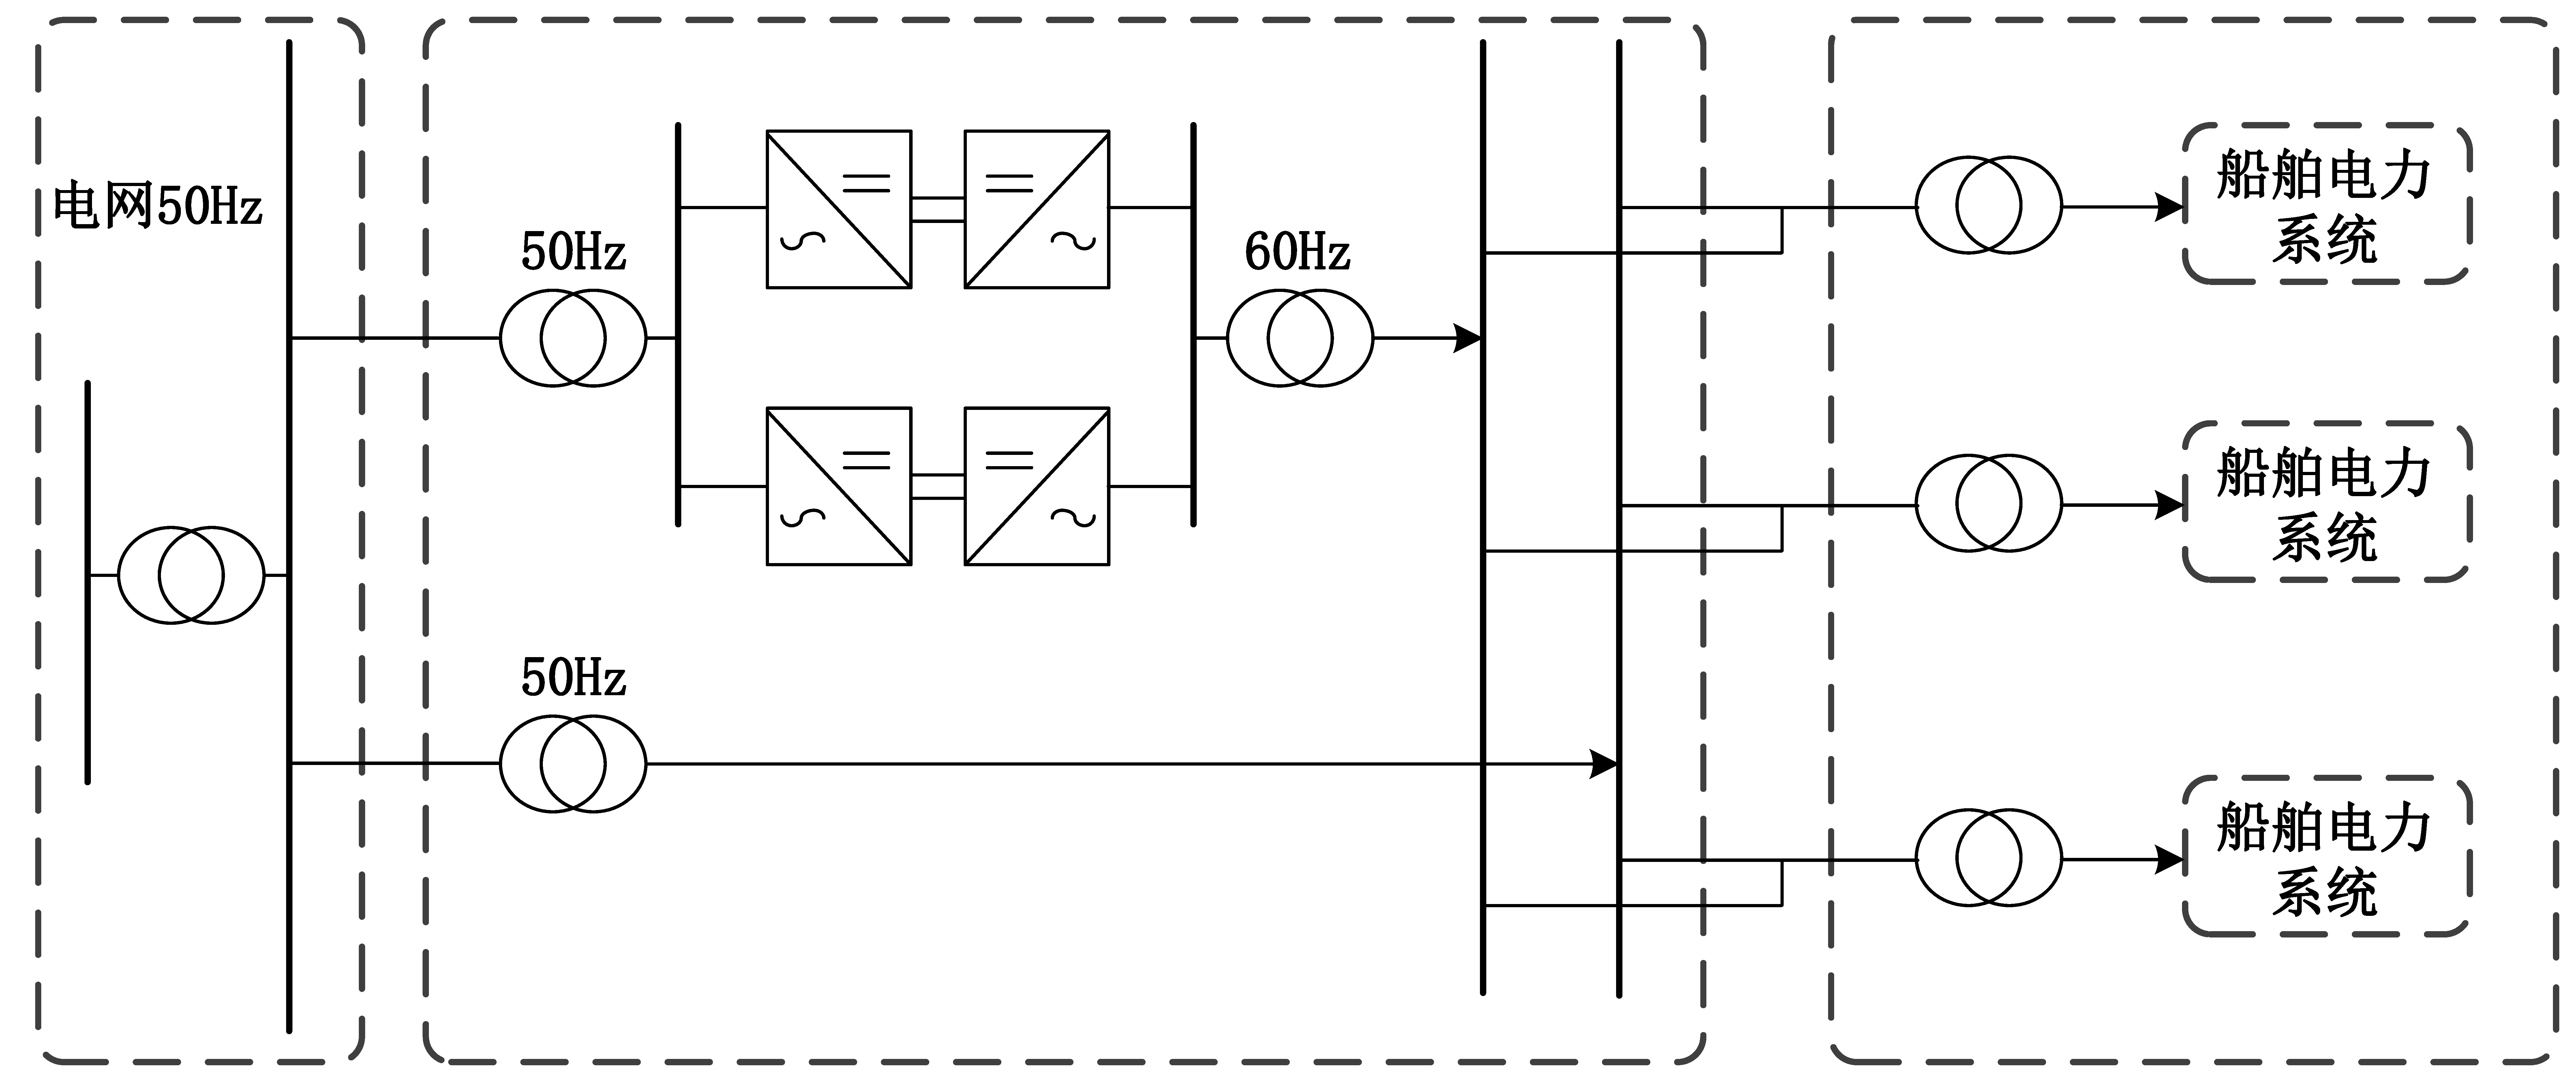
\includegraphics[width=0.85\textwidth]{chapter2/集中式岸电电源.pdf}
	\caption{集中式岸电结构}
	\label{fig:集中式岸电结构}
\end{figure}

\subsection{直流输电式形式}

配置形式如图\ref{fig:直流输电岸电结构}所示,此种配置方式最大特点是,变频设备被分成整流与逆变的两个部分,
采用直流输电。整流器连接港口主变电站的降压变压器,主变电站输出高压直流电,通过电缆连接到泊位的分变电站的
逆变器,直流电经逆变后变为60Hz交流电,最后,经过变压器连接到船舶。
直流传输所占泊位面积较少,系统模块化配置,直流输电电能损耗低。系统容错性低,主变电站的整流器发生故障将影响
整个系统的正常运行,目前直流输电成本比较高,此种电源配置方式应用的水平较低。

\begin{figure}[!htp]
	\centering
	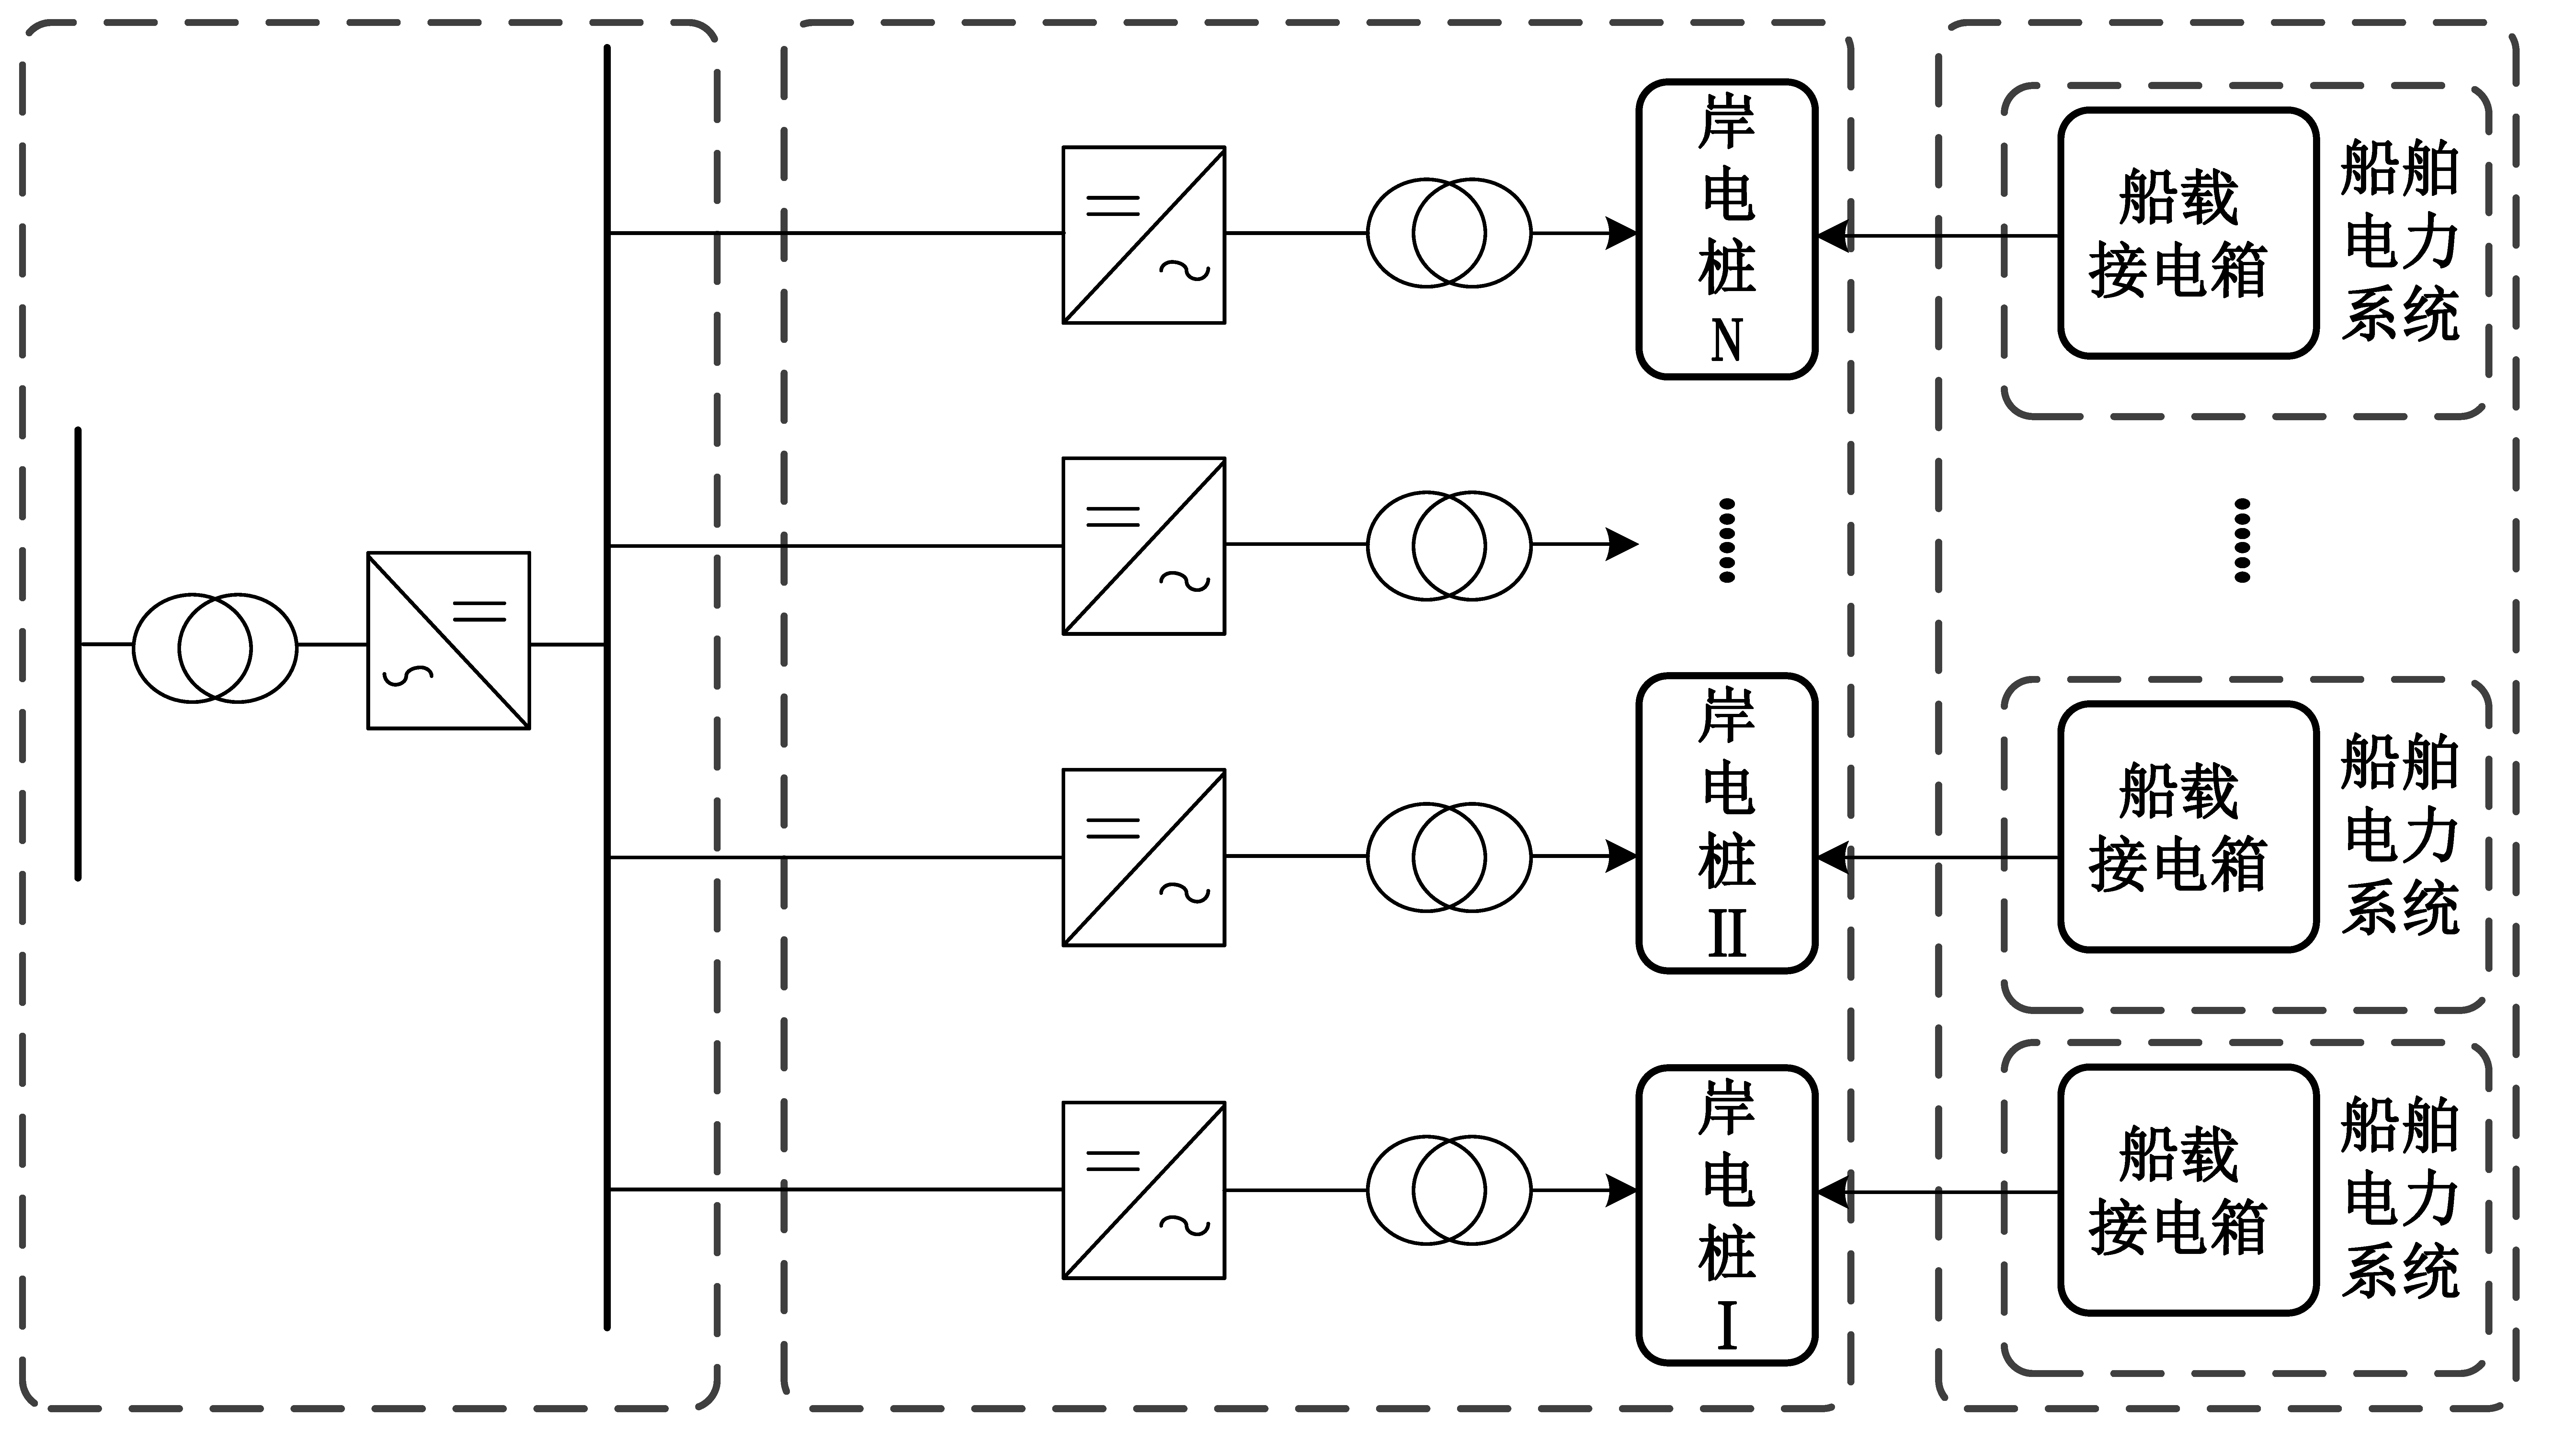
\includegraphics[width=0.85\textwidth]{chapter2/直流输电岸电电源.pdf}
	\caption{直流输电岸电结构}
	\label{fig:直流输电岸电结构}
\end{figure}

\section{本章小结}

本章首先对船岸连接系统的整体组成做了介绍,分析了各个部分的结构,突出了变流装置在系统中的重要性;其次,介绍了
一种高压岸电系统的电气及控制系统的组成及作用;结合数据分析了当前四种主要船舶类型的电制情况,根据用电需求
将岸电系统分为了三类,并详细叙述了其各自组成部分和作用。最后,对三种不同的供电方式和三种不同的电源配置形式进行对比,
发现未来岸电发展的方向是高压岸电,电源配置以集中式为主流。

